\documentclass[11pt]{article}

% --- packages -----------------------------------------------------------------
\usepackage[a4paper, margin=1in]{geometry}
\usepackage{amsmath, amssymb, amsthm, mathtools}
\usepackage{graphicx}
\usepackage{booktabs}
\usepackage{array}
\usepackage{microtype}
\usepackage{xcolor}
\usepackage[most]{tcolorbox}
\usepackage{enumitem}
\usepackage{caption}
\usepackage[numbers, sort&compress]{natbib}
\usepackage{hyperref}

\hypersetup{
  colorlinks=true,
  linkcolor=black!60!blue,
  citecolor=black!60!blue,
  urlcolor=black!50!blue
}

\sloppy
\hbadness=4000
\emergencystretch=3em

% --- theorem environments -----------------------------------------------------
\newtheorem{proposition}{Proposition}
\newtheorem{theorem}[proposition]{Theorem}
\newtheorem{corollary}[proposition]{Corollary}
\newtheorem{lemma}[proposition]{Lemma}

\theoremstyle{definition}
\newtheorem{remark}{Remark}

% --- coloured derivation / interpretation boxes -------------------------------
\definecolor{derivblue}{HTML}{e8f0f8}
\definecolor{derivframe}{HTML}{1a3a5c}
\definecolor{bayesbg}{HTML}{f6efe2}
\definecolor{bayesframe}{HTML}{8a6d2e}
\definecolor{intuibg}{HTML}{e9f1e3}
\definecolor{intuiframe}{HTML}{2f6b34}
\definecolor{auditbg}{HTML}{f1e6ee}
\definecolor{auditframe}{HTML}{6b2356}

\newtcolorbox{derivation}[1][]{
    enhanced, breakable,
    colback=derivblue, colframe=derivframe,
    boxrule=0.6pt, arc=2pt,
    fonttitle=\bfseries, coltitle=white,
    colbacktitle=derivframe,
    attach boxed title to top left={xshift=4pt, yshift=-2pt},
    boxed title style={arc=2pt, boxrule=0pt},
    title={\small Derivation #1},
    left=8pt, right=8pt, top=14pt, bottom=8pt,
}

\newtcolorbox{computation}[1][]{
    enhanced, breakable,
    colback=derivblue, colframe=derivframe,
    boxrule=0.6pt, arc=2pt,
    fonttitle=\bfseries, coltitle=white,
    colbacktitle=derivframe,
    attach boxed title to top left={xshift=4pt, yshift=-2pt},
    boxed title style={arc=2pt, boxrule=0pt},
    title={\small Computation #1},
    left=8pt, right=8pt, top=14pt, bottom=8pt,
}

\newtcolorbox{bayesianview}[1][]{
    enhanced, breakable,
    colback=bayesbg, colframe=bayesframe,
    boxrule=0.6pt, arc=2pt,
    fonttitle=\bfseries, coltitle=white,
    colbacktitle=bayesframe,
    attach boxed title to top left={xshift=4pt, yshift=-2pt},
    boxed title style={arc=2pt, boxrule=0pt},
    title={\small Bayesian view #1},
    left=8pt, right=8pt, top=14pt, bottom=8pt,
}

\newtcolorbox{intuition}[1][]{
    enhanced, breakable,
    colback=intuibg, colframe=intuiframe,
    boxrule=0.6pt, arc=2pt,
    fonttitle=\bfseries, coltitle=white,
    colbacktitle=intuiframe,
    attach boxed title to top left={xshift=4pt, yshift=-2pt},
    boxed title style={arc=2pt, boxrule=0pt},
    title={\small Intuition #1},
    left=8pt, right=8pt, top=14pt, bottom=8pt,
}

\newtcolorbox{auditbox}[1][]{
    enhanced, breakable,
    colback=auditbg, colframe=auditframe,
    boxrule=0.6pt, arc=2pt,
    fonttitle=\bfseries, coltitle=white,
    colbacktitle=auditframe,
    attach boxed title to top left={xshift=4pt, yshift=-2pt},
    boxed title style={arc=2pt, boxrule=0pt},
    title={\small Numerical audit #1},
    left=8pt, right=8pt, top=14pt, bottom=8pt,
}

% --- shorthands ---------------------------------------------------------------
\newcommand{\R}{\mathbb{R}}
\newcommand{\E}{\mathbb{E}}
\newcommand{\Var}{\operatorname{Var}}
\newcommand{\Cov}{\operatorname{Cov}}
\newcommand{\Sig}{\Sigma}
\newcommand{\Detl}{\Delta_t}
\newcommand{\score}{S(x, t)}
\newcommand{\Established}{\textcolor{black!50!green}{\textsf{[Established]}}}
\newcommand{\OpenTag}{\textcolor{black!60!red}{\textsf{[Open]}}}

\title{The Joint Score of Gaussian and Laplace AR(1) Chains \\
       under Ornstein--Uhlenbeck Diffusion \\[6pt]
       \large A unified working note: \\
       Bayesian denoising, belief propagation, and inductive bias}
\author{Giovanni Mantovani \\
        Bocconi University, MSc Data Science \\[2pt]
        \small Supervisors: Prof.\ M.\ M\'ezard (relator) \quad J.\ Garnier-Brun (tutor)}
\date{\today}

\begin{document}
\maketitle

\begin{abstract}
This note consolidates, in a single self-contained reference, the
working programme on the \emph{joint} score
\(S(x, t) = \nabla_x \log P_t(x)\) of a Markov chain corrupted by
independent Ornstein--Uhlenbeck (OU) diffusion. We deliberately
distinguish the joint score from the per-frame marginal score
\(\partial_{x_u} \log p_t(x_u)\): only the joint object inherits the
inter-frame coupling of the Markov prior \(P_0\), and only the joint
object is the right target for the propagator hypothesis at the heart
of the thesis programme.

The narrative arc has three acts. Before they begin, two foundational
chapters establish the language: the score-as-denoiser identity
(Tweedie's lemma) and the Bayesian view of the chain posterior, which
together collapse every score computation to a posterior mean and
every posterior mean to a marginalisation problem. The marginalisation
is then solved by belief propagation on the chain factor graph: a
detailed, from-scratch derivation of the sum--product algorithm,
specialised to Gaussian messages, recovers the Kalman filter and the
Rauch--Tung--Striebel smoother as the forward and backward passes.
\textbf{Act~I} treats the Gaussian AR(1) benchmark in full closed
form: the noised covariance, three equivalent representations of the
noised precision, the spectral preservation theorem, the band-fill
lifecycle, and the \(O(K)\) belief-propagation / Kalman smoother
that recovers the exact joint score. \textbf{Act~II} is the Laplace
warm-up at \(K = 1\), where Gaussianity is broken while Markovianity
is structurally absent; the joint score acquires nonlinearity but
Tweedie's identity carries through unchanged. \textbf{Act~III}
promotes Laplace innovations to \(K \geq 2\), retaining the chain
factor graph: belief propagation is still exact in principle, the
forward message admits a clean closed form, the backward message
exhibits a fundamental causal asymmetry, and the remaining structural
questions are listed explicitly. The note closes with an
information-theoretic argument for why the factor-graph
parametrisation should be a more informative prior with respect to a black-box neural approximator: it encodes the Markov prior as architectural inductive
bias, in analogy with the role of locality and weight-sharing
in convolutional networks. Every quantitative claim carries either an
\Established\ tag (proved and numerically verified at the tolerances
of \texttt{numerical\_audit.py}) or an \OpenTag\ tag.
\end{abstract}

\tableofcontents


% =============================================================================
\section{Introduction and Motivation}\label{sec:intro}
% =============================================================================

\paragraph{What generative diffusion is.} Generative diffusion is a
very active field of research. In a nutshell, it aims at generating
artificial data \(a \in \R^d\) drawn from a distribution \(P_0(a)\)
which is not known explicitly, but for which we have a database of
\(n\) examples \(a^{\mu}\), \(\mu \in \{1, \dots, n\}\), supposed to be
iid samples of \(P_0\). Notice that \(P_0\) itself is usually not well
defined (think of generating images of non-existent celebrities). As
we will see, generative diffusion allows one to train a system with a
two-step procedure: first \emph{noising} the data through a diffusion
process in \(\R^d\), then \emph{denoising} the result through another
diffusion process with a guiding force field --- the \emph{score} ---
trained from the data, so that the system generates fresh fake data
with properties similar to the originals
\citep{Mezard2025, SohlDickstein2015, Ho2020, Song2021SDE,
Karras2022, Achilli2024}. This is presently the state of the art in
image, text, and video generation.
The same formalism can also be used to estimate the likelihood
\(\log P_0(x)\) of a new point \(x\), using the score obtained from
training the generative model
\citep{Song2021SDE}.

\paragraph{Our setting: dynamic objects.} This thesis studies
score-based diffusion models applied to \emph{dynamic objects}: data
that arise as ordered sequences with a non-trivial internal time, the
canonical example being a short video clip. A dynamic object is a
sequence of \(K\) frames \(a_0, a_1, \dots, a_{K-1} \in \R^d\), indexed by
internal time \(u = 0, \dots, K-1\), drawn from a clean joint distribution
\(P_0(a_0, \dots, a_{K-1})\) that encodes the temporal dependence of the
data. Throughout this thesis we assume that the prior has \emph{Markov
structure}: consecutive frames are coupled through a transition kernel
\(M(a_{u+1} \mid a_u)\), so that
\begin{equation}\label{eq:chain-prior}
    P_0(a_0, \dots, a_{K-1})
    \;=\;
    p_0(a_0)\, \prod_{u=0}^{K-2} M(a_{u+1} \mid a_u).
\end{equation}
The diffusion paradigm corrupts the data by applying an independent
Ornstein--Uhlenbeck (OU) process to each frame. As we derive in
Section~\ref{sec:setup}, the resulting forward channel at noise time \(t\)
is the affine Gaussian map
\(x_u = \mu\, a_u + \sqrt{\Detl}\, \xi_u\) with
\(\mu = e^{-t}\), \(\Detl = 1 - e^{-2t}\), and
\(\xi_u \stackrel{\text{iid}}{\sim} \mathcal N(0, 1)\). Sampling from
\(P_0\) reduces, by Anderson's time-reversal theorem
\citep{Anderson1982, HaussmannPardoux1986}, to running a
reverse-time SDE whose drift contains the \emph{joint score field}
\begin{equation}\label{eq:joint-score-def}
    \mathbf S(x, t)
    \;:=\;
    \nabla_x \log P_t(x_0, \dots, x_{K-1})
    \;\in\; \R^{dK}.
\end{equation}
The \(k\)-th block component admits the exact posterior-mean representation
\begin{equation}\label{eq:tweedie-preview}
    S_k(x, t)
    \;=\;
    \frac{\mu\, \E[a_k \mid x_0, \dots, x_{K-1}] - x_k}{\Detl},
\end{equation}
and is emphatically \emph{not} the per-frame marginal score
\(\nabla_{x_k} \log p_t(x_k)\): the latter integrates out every frame
other than \(x_k\), treating the sequence as if it had been generated
frame-by-frame independently. The joint score instead couples every
frame to the entire trajectory through the full posterior
\(P(a_0, \dots, a_{K-1} \mid x_0, \dots, x_{K-1})\).

The central question of this thesis is therefore: \emph{what structure
does \(\mathbf S(x, t)\) inherit from the Markov factorisation
\eqref{eq:chain-prior} of \(P_0\), and can that structure be exploited
to design more principled and computationally efficient score
architectures for dynamic data?}

Two observations motivate everything that follows.

\begin{intuition}[Score and denoising are the same problem]
The posterior-mean representation \eqref{eq:tweedie-preview} is
\emph{Tweedie's identity}, and it says more than that the score admits a
closed form: it says that learning the score \(\mathbf S(x, t)\) and
learning the Bayes-optimal denoiser \(x \mapsto \E[a \mid x]\) are
\emph{mathematically the same problem}, related by an affine,
prior-independent rescaling. Two consequences follow at once. First, the
prior \(P_0\) enters the score \emph{only} through the conditional
expectation, so every structural property of \(\E[a \mid x]\) ---
linearity, locality, factorisation --- is inherited by \(\mathbf S\).
Second, the score is linear in \(x\) if and only if the Bayes denoiser
is linear in \(x\); the question of when diffusion models admit affine
score fields therefore reduces to the classical question of when the
posterior mean is affine in the observation, with its clean Gaussian
answer.
\end{intuition}

\begin{intuition}[Inductive bias is structure, not training data]
For a Markov chain prior \eqref{eq:chain-prior}, \(P_0\) factorises over
nearest-neighbour pairs and the OU likelihood factorises over single
frames (\S\ref{sec:setup}). The posterior \(P(a \mid x)\) is therefore a
tree-structured graphical model, on which belief propagation is exact
in \(O(K)\) message-passing operations. A neural network parametrising
the score blindly re-discovers this graph from data; a factor-graph
parametrisation \emph{is} this graph. The inductive bias is the same
shift that took convolutional networks from generic MLPs: encoding what
we already know about the data into the architecture, instead of
spending capacity learning it from samples.
\end{intuition}

The two ideas are connected: the score is a posterior expectation, the
posterior factorises like the prior, and belief propagation is the
algorithm that exploits that factorisation. The remainder of this note
works the connection out in detail. Section~\ref{sec:setup} fixes
notation and derives the forward channel from the OU SDE; sections
\ref{sec:tweedie} and \ref{sec:bayesian} establish the score-as-denoiser
identity and the Bayesian view of the chain posterior;
section~\ref{sec:factor-graph} draws the factor graph;
section~\ref{sec:bp} derives belief propagation from sum--product on
trees and identifies the Gaussian case with the Kalman smoother;
section~\ref{sec:gaussian} executes the Gaussian AR(1) benchmark in full
closed form; sections \ref{sec:K1} and \ref{sec:K2} push the Laplace
generalisation to \(K = 1\) and \(K \geq 2\); section~\ref{sec:audit}
reports the audit; section~\ref{sec:inductive-bias} makes the
inductive-bias case explicit.

% =============================================================================
\section{Setup, notation, and the OU forward channel}\label{sec:setup}
% =============================================================================

\paragraph{Clean dynamics.} We work in the scalar-frame setting
\(d = 1\); the construction is per-component and extends without
change to \(d > 1\). A dynamic object is then
\(a = (a_0, \dots, a_{K-1}) \in \R^K\) drawn from the Markov chain
\eqref{eq:chain-prior}. We specialise to two cases:
\begin{itemize}[leftmargin=1.8em]
    \item \emph{Gaussian AR(1)}: \(a_{u+1} = \alpha a_u + \eta_u\) with
        \(\eta_u \sim \mathcal N(0, \sigma_\eta^2)\);
    \item \emph{Laplace AR(1)}: \(a_{u+1} = \alpha a_u + \eta_u\) with
        \(\eta_u \sim \mathrm{Laplace}(0, b)\).
\end{itemize}
In both cases \(|\alpha| < 1\) and the law of \(a_0\) is fixed to
enforce stationarity. For Gaussian AR(1) this gives the standard
relation
\(\sigma_0^2 = \sigma_\eta^2 / (1 - \alpha^2)\) between the
innovation variance and the initial variance, so that
\(\Var(a_u) = \sigma_0^2\) for every \(u\). When we plot or audit
numerically we adopt the unit-variance normalisation
\(\sigma_0^2 = 1\), so that \(\sigma_\eta^2 = 1 - \alpha^2\); the
notation table reflects this normalisation.

\paragraph{Forward channel.} Each frame is independently corrupted by the
variance-preserving OU SDE \citep{UhlenbeckOrnstein1930, Oksendal2003}
\begin{equation}\label{eq:ou-sde}
    \mathrm d x_{u,t}
    \;=\; -x_{u,t}\, \mathrm d t
    \;+\; \sqrt{2}\, \mathrm d W_{u,t},
    \qquad
    x_{u,0} = a_u,
    \qquad
    u = 0, \dots, K-1,
\end{equation}
where \(\{W_{u, \cdot}\}_{u=0}^{K-1}\) are mutually independent standard
Brownian motions. The closed-form transition is obtained by an
integrating-factor argument, which we now carry out in full.

\begin{derivation}[from the OU SDE \eqref{eq:ou-sde} to the closed-form
transition]
We drop the frame index \(u\) for the moment; the result applies
coordinate-wise and the cross-frame independence is reinstated at the end.

\medskip\noindent
\textsc{Step 1 (integrating factor).}
The deterministic ODE \(\dot x = -x\) has solution \(x(t) = x_0 e^{-t}\).
This suggests rescaling the process by \(e^t\) to absorb the drift.
Define
\begin{equation}
    y_t \;:=\; e^{t}\, x_t.
\end{equation}
We will show that \(y_t\) is a pure It\^o integral, with no drift; then we
read off \(x_t\) by inversion.

\medskip\noindent
\textsc{Step 2 (apply It\^o's lemma to \(y_t = f(t, x_t)\) with
\(f(t, x) = e^t x\)).}
The partial derivatives are
\begin{equation}
    \partial_t f \;=\; e^t x,
    \qquad
    \partial_x f \;=\; e^t,
    \qquad
    \partial_{xx} f \;=\; 0.
\end{equation}
It\^o's formula reads
\(\mathrm d y_t = \partial_t f\, \mathrm d t
   + \partial_x f\, \mathrm d x_t
   + \tfrac{1}{2}\, \partial_{xx} f\, (\mathrm d x_t)^2\).
Since \(\partial_{xx} f = 0\) the It\^o correction vanishes, and substituting
the SDE \eqref{eq:ou-sde} for \(\mathrm d x_t\) gives
\begin{align}
    \mathrm d y_t
        &= e^{t} x_t\, \mathrm d t
            + e^{t}\bigl(-x_t\, \mathrm d t + \sqrt{2}\, \mathrm d W_t\bigr)
            \notag \\
        &= \underbrace{e^t x_t\, \mathrm d t - e^t x_t\, \mathrm d t}_{=\,0}
            + \sqrt{2}\, e^{t}\, \mathrm d W_t
            \notag \\
        &= \sqrt{2}\, e^{t}\, \mathrm d W_t.
        \label{eq:dy-pure-noise}
\end{align}
The drift cancels by construction --- this is the entire purpose of the
rescaling. The transformed process \(y_t\) is a pure Wiener integral.

\medskip\noindent
\textsc{Step 3 (integrate from \(0\) to \(t\)).}
The initial condition is \(y_0 = e^{0} x_0 = a\). Integrating
\eqref{eq:dy-pure-noise},
\begin{equation}\label{eq:yt-integrated}
    y_t \;=\; a \;+\; \sqrt{2}\, \int_{0}^{t} e^{s}\, \mathrm d W_s.
\end{equation}
Multiplying both sides by \(e^{-t}\) and using \(x_t = e^{-t} y_t\),
\begin{equation}\label{eq:xt-explicit}
    x_t \;=\; e^{-t}\, a
    \;+\; \sqrt{2}\, \int_{0}^{t} e^{-(t - s)}\, \mathrm d W_s.
\end{equation}
This is the explicit solution: a deterministic exponential decay of the
initial condition, plus a stochastic integral against the OU kernel
\(e^{-(t - s)}\).

\medskip\noindent
\textsc{Step 4 (identify the law of the stochastic integral).}
Write
\begin{equation}
    I_t \;:=\; \sqrt{2}\, \int_{0}^{t} e^{-(t - s)}\, \mathrm d W_s.
\end{equation}
Since the integrand \(s \mapsto \sqrt{2}\, e^{-(t - s)}\) is deterministic,
\(I_t\) is a Wiener integral of a deterministic function, hence centred
Gaussian. Its variance is given by It\^o's isometry,
\(\E\!\left[\bigl(\int_0^t f(s)\, \mathrm d W_s\bigr)^{2}\right] = \int_0^t
f(s)^2\, \mathrm d s\), so
\begin{equation}
    \Var(I_t)
    \;=\; \int_{0}^{t} \bigl(\sqrt{2}\, e^{-(t - s)}\bigr)^2 \mathrm d s
    \;=\; 2 \int_{0}^{t} e^{-2 (t - s)}\, \mathrm d s.
\end{equation}
Evaluate the remaining integral by the substitution
\(u = t - s, \mathrm d u = -\mathrm d s\), which sends
\(s = 0 \to u = t\) and \(s = t \to u = 0\):
\begin{equation}
    \int_{0}^{t} e^{-2 (t - s)}\, \mathrm d s
    \;=\; \int_{t}^{0} e^{-2 u}\, (-\mathrm d u)
    \;=\; \int_{0}^{t} e^{-2 u}\, \mathrm d u
    \;=\; \frac{1 - e^{-2 t}}{2}.
\end{equation}
Multiplying by \(2\),
\begin{equation}
    \Var(I_t) \;=\; 1 - e^{-2 t}.
\end{equation}

\medskip\noindent
\textsc{Step 5 (standardise).}
Define the noise variance
\begin{equation}
    \Detl \;:=\; 1 - e^{-2 t},
\end{equation}
and write \(I_t = \sqrt{\Detl}\, \xi\) with \(\xi \sim \mathcal N(0, 1)\).
Combining with \eqref{eq:xt-explicit} gives the closed-form transition:
\begin{equation}\label{eq:forward-channel}
    \boxed{\;\;
    x_{u, t} \;=\; \mu\, a_u \;+\; \sqrt{\Detl}\, \xi_u,
    \qquad
    \mu := e^{-t},
    \qquad
    \xi_u \stackrel{\text{iid}}{\sim} \mathcal N(0, 1).
    \;\;}
\end{equation}

\medskip\noindent
\textsc{Step 6 (independence across frames).}
Because the SDEs \eqref{eq:ou-sde} are driven by independent Brownian
motions \(\{W_{u, \cdot}\}_{u = 0}^{K - 1}\), the noises
\(\{\xi_u\}_{u = 0}^{K - 1}\) appearing in \eqref{eq:forward-channel} are
mutually independent. The full forward map \(a \mapsto x\) is therefore an
iid affine Gaussian channel applied to each coordinate.

\medskip\noindent
\textsc{Why ``variance-preserving''.}
For data of unit clean variance \(\Var(a) = 1\), the channel
\eqref{eq:forward-channel} yields
\(\Var(x_t) = \mu^2 \cdot 1 + \Detl = e^{-2 t} + (1 - e^{-2 t}) = 1\) for
all \(t \geq 0\). The marginal variance of \(x_t\) is exactly preserved,
which is the standard sense in which \eqref{eq:ou-sde} is called the
variance-preserving SDE (as opposed to ``variance-exploding'' pure
Brownian motion). \qed
\end{derivation}

\paragraph{Likelihood factorisation.} Since each frame's OU process is
independent of the others, the likelihood factorises across frames:
\begin{equation}\label{eq:likelihood}
    p(x \mid a)
    \;=\; \prod_{k = 0}^{K - 1} p_t(x_k \mid a_k),
    \qquad
    p_t(x_k \mid a_k)
    \;=\; \mathcal N\!\bigl(x_k;\, \mu\, a_k,\, \Detl\bigr).
\end{equation}
This is the second structural feature of the model: the prior is Markov
along \(u\), the likelihood is product-form across \(u\). The non-trivial
inter-frame coupling of the posterior \(P(a \mid x)\) therefore comes
\emph{entirely} from the prior; the channel itself introduces none.

\paragraph{The joint score, formally.} Combining \eqref{eq:chain-prior}
and \eqref{eq:likelihood}, the noised joint density of
\eqref{eq:joint-score-def} admits the integral representation
\begin{equation}\label{eq:Pt-integral}
    P_t(x)
    \;=\;
    \int_{\R^{K}} P_0(a)\, p(x \mid a)\, \mathrm d a
    \;=\;
    \int_{\R^{K}} P_0(a)\,
    \prod_{k = 0}^{K - 1}
    \mathcal N\!\bigl(x_k;\, \mu\, a_k,\, \Detl\bigr)\, \mathrm d a.
\end{equation}
The \(k\)-th component of the joint score
\eqref{eq:joint-score-def} is the partial derivative
\(S_k(x, t) = \partial_{x_k} \log P_t(x)\), taken holding \emph{all
other frames \(x_{j \neq k}\) fixed}. This is the technical content of
the joint-versus-marginal distinction: \(S_k\) is a function of the
entire noisy trajectory, not of \(x_k\) alone.

\begin{bayesianview}[: the Fokker--Planck view of the forward process]
The forward channel \eqref{eq:ou-sde} can equivalently be characterised
by the evolution of the density \(P_t(x)\) itself, which solves the
\emph{Fokker--Planck equation} \citep[][\S\,2]{Mezard2025}
\begin{equation}\label{eq:fpe-forward}
    \partial_t P_t(x)
    \;=\;
    \nabla_x \cdot \bigl(x\, P_t(x)\bigr)
    \;+\;
    \Delta_x P_t(x).
\end{equation}
The first term is the drift contribution from the restoring force
\(-x\); the second is the diffusion contribution from the white noise.
The integral form \eqref{eq:Pt-integral} is the explicit solution of
\eqref{eq:fpe-forward} with initial condition
\(P_{t = 0} = P_0\): the Gaussian factor
\(\mathcal N(x_k; \mu a_k, \Detl)\) is precisely the Green's function
of the OU Fokker--Planck operator. Two facts will matter later: at
\(t \to \infty\), the steady-state solution of \eqref{eq:fpe-forward}
is the standard Gaussian
\(P_{\infty}(x) = (2 \pi)^{-K/2} e^{-\|x\|^2 / 2}\) (the
``\emph{easy distribution}'' from which reverse-time sampling
starts); and the \(\nabla_x \log P_t\) gradient that appears as a
correction to the drift when one time-reverses the Fokker--Planck
equation is exactly the score \citep[][\S\,3.1]{Mezard2025,
Anderson1982} which the rest of this note studies.
\end{bayesianview}


\paragraph{Notation.}
\begin{center}
\small
\setlength{\tabcolsep}{8pt}
\begin{tabular}{@{}>{\(}l<{\)}p{0.40\linewidth}p{0.30\linewidth}@{}}
\toprule
\multicolumn{1}{@{}l}{Symbol} & Meaning & Note \\
\midrule
K          & sequence length & \\
a_k        & clean frame at internal time \(k\) & \\
x_k        & noisy observation at \(t\) & \\
\alpha     & AR(1) coefficient & \(|\alpha| < 1\) \\
\sigma_\eta & Gaussian innovation std & \(\sqrt{1 - \alpha^2}\)
                                        at \(\sigma_0^2 = 1\) \\
\sigma_0    & initial std of \(a_0\) & stationary: \(\sigma_0^2 =
                                        \sigma_\eta^2 / (1 - \alpha^2)\) \\
\mu_0      & initial mean of \(a_0\) & zero in the stationary case \\
b          & Laplace innovation scale & \\
\mu = e^{-t} & OU signal-attenuation factor & \\
\Detl = 1 - e^{-2 t} & OU noise variance & \\
P_0,\, p_0,\, M & prior, frame-0 marginal, transition & \\
P_t,\, p_t & noised joint and marginal & \\
\mu_a       & prior mean vector & \(\mu_a[k] = \alpha^k \mu_0\) \\
\Sig_0     & joint clean covariance & Gaussian case \\
Q_0 = \Sig_0^{-1} & joint clean precision & tridiagonal for AR(1) \\
\Sig_t = \mu^2 \Sig_0 + \Detl I & joint noised covariance & \\
Q_t = \Sig_t^{-1} & joint noised precision & \\
S(x, t)    & \emph{joint} score \(\nabla_x \log P_t(x)\) & \\
s(x_u, u, t) & per-frame marginal score & \emph{no inter-correlations} \\
\bottomrule
\end{tabular}
\end{center}

% =============================================================================
\section{The score is a denoiser: Tweedie's identity}\label{sec:tweedie}
% =============================================================================

The fundamental identity that organises every score computation in
this note is Tweedie's lemma, in its joint form
\citep{Efron2011, Thiery2023}. Its content is simple and remarkable:
the score field is an affine map of the Bayes-optimal denoiser
\(\E[a \mid x]\). The prior \(P_0\) enters only through this
conditional expectation; the Gaussian channel contributes only the
affine constants \(\mu = e^{-t}\) and \(\Detl = 1 - e^{-2t}\).
Computing the score and computing the Bayesian denoiser are therefore
the same problem; in the OU setting of this thesis the same identity
appears in \cite[\S\,3]{Mezard2025} and is the foundation of denoising
score matching \citep{Vincent2011}.

\begin{theorem}[Joint Tweedie identity, \Established; cf.\
\cite{Efron2011, Thiery2023}]\label{thm:tweedie}
Let \(P_0\) be any prior on \(\R^K\), let \(t > 0\), and write the
joint noised density induced by the forward channel
\eqref{eq:forward-channel} as
\begin{equation}\label{eq:Pt-def}
    P_t(x)
    \;=\;
    \int_{\R^K} P_0(a)\, p(x \mid a)\, \mathrm d a,
    \qquad
    p(x \mid a)
    \;=\;
    \prod_{k=0}^{K-1}
    \frac{1}{\sqrt{2\pi \Detl}}
    \exp\!\Bigl(-\tfrac{(x_k - \mu a_k)^2}{2 \Detl}\Bigr).
\end{equation}
Then the joint score \(\score(x, t) := \nabla_x \log P_t(x)\) admits,
component-wise, the two equivalent forms
\begin{equation}\label{eq:tweedie}
    S_k(x, t)
        \;=\; \frac{\mu\, \E[a_k \mid x] - x_k}{\Detl}
        \;=\; -\,\frac{\E[\xi_k \mid x]}{\sqrt{\Detl}},
    \qquad k = 0, \dots, K - 1,
\end{equation}
where the conditional expectation is taken under the posterior
\(P(a \mid x)\), and \(\xi\) is the standard Gaussian noise of the
channel decomposition \(x = \mu\, a + \sqrt{\Detl}\, \xi\).
\end{theorem}

\begin{derivation}[\ref*{thm:tweedie}: from the channel to Tweedie]
The proof structure follows \cite[\S\,2]{Thiery2023}, adapted from the
pure Brownian channel to the variance-preserving OU channel
\eqref{eq:forward-channel}. The score is, by definition, the gradient
of a log-density, and the log-gradient of any positive function
\(f\) satisfies the elementary identity
\begin{equation}\label{eq:log-grad}
    \nabla_x \log f(x) \;=\; \frac{\nabla_x f(x)}{f(x)}.
\end{equation}
Applied to \(P_t\), this turns the computation of the score into
the computation of \(\partial_{x_k} P_t(x)\) divided by \(P_t(x)\),
which is what we now do.

Start from the integral expression \eqref{eq:Pt-def} for \(P_t(x)\)
and differentiate with respect to \(x_k\). Because the prior \(P_0(a)\)
does not depend on \(x\), the derivative passes inside the integral
and acts only on the Gaussian likelihood \(p(x \mid a)\):
\begin{equation}\label{eq:dPt-1}
    \partial_{x_k} P_t(x)
    \;=\;
    \int_{\R^K} P_0(a)\;
    \partial_{x_k} p(x \mid a) \; \mathrm d a.
\end{equation}
The Gaussian likelihood is itself an exponential of a quadratic in
\(x_k\), so its \(x_k\)-derivative is explicit. Writing
\(\log p(x \mid a)
= -\frac{(x_k - \mu a_k)^2}{2 \Detl} + (\text{terms independent of }x_k)\)
and differentiating,
\begin{equation}\label{eq:gauss-deriv}
    \partial_{x_k} p(x \mid a)
    \;=\;
    -\frac{x_k - \mu\, a_k}{\Detl}\; p(x \mid a).
\end{equation}
The interpretation is already visible at this point: the gradient of
the Gaussian channel is the channel itself, multiplied by the
``displacement from the channel mean'' \((x_k - \mu a_k)\), with the
expected minus sign and the variance \(\Detl\) in the denominator.

Substitute \eqref{eq:gauss-deriv} into \eqref{eq:dPt-1}:
\begin{equation}\label{eq:dPt-2}
    \partial_{x_k} P_t(x)
    \;=\;
    -\,\frac{1}{\Detl}\,
    \int_{\R^K}
    (x_k - \mu\, a_k)\; P_0(a)\, p(x \mid a)\; \mathrm d a.
\end{equation}
The factor \(x_k\) does not depend on \(a\) and can be pulled
outside the integral; the remaining integral of \(P_0(a)\, p(x \mid a)\)
is, by \eqref{eq:Pt-def}, just \(P_t(x)\). The integral involving
\(a_k\) is the object we must understand:
\begin{equation}
    \partial_{x_k} P_t(x)
    \;=\;
    -\,\frac{1}{\Detl}
    \Bigl[\,
        x_k\, P_t(x)
        \;-\;
        \mu
        \int_{\R^K}
        a_k\, P_0(a)\, p(x \mid a)\; \mathrm d a
    \Bigr].
\end{equation}

This is the point at which Bayes' theorem enters. The joint density of
the clean--noisy pair is \(P_0(a)\, p(x \mid a)\), and dividing by
its marginal \(P_t(x)\) gives the posterior:
\begin{equation}\label{eq:bayes}
    P(a \mid x)
    \;=\;
    \frac{P_0(a)\, p(x \mid a)}{P_t(x)}.
\end{equation}
Dividing \(\partial_{x_k} P_t(x)\) by \(P_t(x)\) is therefore the same
as taking the expectation of \((x_k - \mu a_k)\) under \(P(a \mid x)\),
up to the factor \(-1/\Detl\):
\begin{equation}\label{eq:after-bayes}
    \frac{\partial_{x_k} P_t(x)}{P_t(x)}
    \;=\;
    -\,\frac{1}{\Detl}
    \int_{\R^K}
    (x_k - \mu\, a_k)\, P(a \mid x)\, \mathrm d a
    \;=\;
    -\,\frac{x_k - \mu\, \E[a_k \mid x]}{\Detl}.
\end{equation}
In the last step we used linearity of the integral, the fact that
\(P(a \mid x)\) is a probability measure (so that \(x_k\) integrates
out to \(x_k\)), and the definition of the conditional expectation
\(\E[a_k \mid x] = \int a_k\, P(a \mid x)\, \mathrm d a\).

By the log-gradient identity \eqref{eq:log-grad}, the left-hand side of
\eqref{eq:after-bayes} is exactly the \(k\)-th component \(S_k(x, t)\)
of the joint score. Rearranging,
\begin{equation}\label{eq:tweedie-first}
    S_k(x, t)
    \;=\;
    \frac{\mu\, \E[a_k \mid x] - x_k}{\Detl},
\end{equation}
which is the first form announced in \eqref{eq:tweedie}.

The second, ``noise-form'' identity is now a one-line rewriting of the
first. The forward channel decomposes as
\(x = \mu\, a + \sqrt{\Detl}\, \xi\), with \(\xi \sim \mathcal N(0, I)\)
independent of \(a\); equivalently, on the joint space,
\(\xi_k = (x_k - \mu\, a_k) / \sqrt{\Detl}\). Conditioning on \(x\) and
taking expectations of both sides --- noting that \(x_k\) is a function
of \(x\) and so passes through the conditional expectation unchanged ---
yields
\begin{equation}
    \E[\xi_k \mid x]
    \;=\;
    \frac{x_k - \mu\, \E[a_k \mid x]}{\sqrt{\Detl}}.
\end{equation}
Comparing with \eqref{eq:tweedie-first}, the right-hand side equals
\(-\sqrt{\Detl}\, S_k(x, t)\), so
\begin{equation}
    S_k(x, t)
    \;=\;
    -\,\frac{\E[\xi_k \mid x]}{\sqrt{\Detl}},
\end{equation}
which is the second form in \eqref{eq:tweedie}. \qed
\end{derivation}

\subsection{Three readings of the same identity}\label{sec:tweedie-readings}

The two equivalent forms of \eqref{eq:tweedie} carry three
operational readings. The first reading is the \emph{denoiser
identity}: the score is, up to known channel constants, the affine
correction that converts the noisy observation into the Bayes-optimal
estimate of the clean signal. The second reading is the
\emph{posterior expected noise} interpretation, which is what the
reverse-time SDE actually adds back during sampling. The third
reading -- the one that organises the rest of this note -- is that the
prior \(P_0\) enters the score only through the conditional
expectation \(\E[a \mid x]\), so every structural property of the
score (linearity, factorisation, sparsity) is inherited from the
structure of the Bayesian denoiser.

\begin{bayesianview}[: the score \emph{is} the optimal denoiser]
Solving \eqref{eq:tweedie} for the conditional expectation,
\begin{equation}\label{eq:denoiser-from-score}
    \E[a \mid x] \;=\; \frac{x + \Detl\, S(x, t)}{\mu}.
\end{equation}
The Bayes-optimal denoiser at every time \(t\) is an affine function
of the score with known coefficients. Knowing the score and knowing
the optimal denoiser are exactly the same problem; everything below is
ultimately a strategy for computing
\(\E[a \mid x]\) and reading off \(\score\) from
\eqref{eq:denoiser-from-score}.
\end{bayesianview}

\begin{bayesianview}[: the score is the posterior expected noise]
The second form in \eqref{eq:tweedie} reads
\(\score = -\E[\xi \mid x] / \sqrt{\Detl}\). Up to the channel
scaling \(\sqrt{\Detl}\), the score is the conditional expectation
of the corruption noise given the observation. The reverse-time
generative SDE
\eqref{eq:reverse-sde}, derived below, therefore literally ``adds
back twice the expected noise'': diffusion sampling is the sequential
cancellation of the corruption that the forward channel injected
\citep{Anderson1982, Song2021SDE, Ho2020}.
\end{bayesianview}

\begin{derivation}[from forward FPE to backward SDE: where the score
enters as drift]
The reverse-time SDE alluded to above is a special case of Anderson's
general theorem on time reversal of diffusions \citep{Anderson1982,
HaussmannPardoux1986}. We sketch the OU case to make explicit how the
score appears \citep[][\S\,3.1]{Mezard2025}.

\textbf{Step 1 (write the FPE in reversed time).} The forward
Fokker--Planck \eqref{eq:fpe-forward} reads
\(\partial_t P_t = \nabla \cdot (x P_t) + \Delta P_t\) and governs
the evolution of the noised density forward in time. Define the
reverse-time variable \(\tau := t_f - t\) and the reverse-time density
\(\widetilde P_\tau(x) := P_{t_f - \tau}(x)\). Then
\(\partial_\tau \widetilde P_\tau = -\partial_t P_{t_f - \tau}\),
which after substituting \eqref{eq:fpe-forward} gives
\begin{equation}\label{eq:fpe-reversed-raw}
    \partial_\tau \widetilde P_\tau(x)
    \;=\;
    -\nabla \cdot \bigl(x\, \widetilde P_\tau(x)\bigr)
    \;-\; \Delta \widetilde P_\tau(x).
\end{equation}
This is \emph{not} the FPE of a forward Langevin equation: the
diffusion term has the wrong sign.

\textbf{Step 2 (replace one Laplacian by a score-drift).} Note that
\(\nabla \widetilde P_\tau = (\nabla \log \widetilde P_\tau)\,
\widetilde P_\tau\), so
\(\Delta \widetilde P_\tau = \nabla \cdot \bigl( (\nabla \log
\widetilde P_\tau)\, \widetilde P_\tau \bigr)\). Adding and
subtracting one copy of \(\Delta \widetilde P_\tau\) -- i.e.\ using
the identity \(A = 2 A - A\) with
\(A = \Delta \widetilde P_\tau\) and substituting the score
expression for the first copy -- rewrites the wrong-sign Laplacian as
\begin{equation}\label{eq:laplacian-split}
    -\Delta \widetilde P_\tau
    \;=\;
    \underbrace{-\, 2\, \nabla \cdot \bigl(
        (\nabla \log \widetilde P_\tau)\, \widetilde P_\tau
    \bigr)}_{\text{a new drift term}}
    \;+\;
    \underbrace{\Delta \widetilde P_\tau}_{\text{Laplacian, now with the right sign}}.
\end{equation}
No new information has entered \eqref{eq:laplacian-split}: it is the
identity \(A = 2 A - A\) with one of the two \(A\)'s rewritten via
\(\Delta P = \nabla \cdot ((\nabla \log P)\, P)\). Its purpose is
\emph{purely structural} -- it splits the wrong-sign diffusion of
Step~1 into a drift term plus a right-sign diffusion term, exposing
exactly which extra drift is needed to convert the reversed FPE into
that of a forward Langevin equation.

\textbf{Step 3 (collect).} Substituting \eqref{eq:laplacian-split}
into \eqref{eq:fpe-reversed-raw} gives the FPE
\begin{equation}\label{eq:fpe-backward}
    \partial_\tau \widetilde P_\tau(x)
    \;=\;
    -\nabla \cdot \!\bigl[\, \bigl(\, x +
        2\, \nabla \log \widetilde P_\tau(x) \,\bigr)\,
        \widetilde P_\tau(x) \,\bigr]
    \;+\;
    \Delta \widetilde P_\tau(x).
\end{equation}
The right-hand side is now the FPE of a forward Langevin equation in
the variable \(\tau\), with drift
\(\,x + 2\, \nabla \log \widetilde P_\tau(x)\,\) and the standard
diffusion. Reading off the corresponding SDE,
\begin{equation}\label{eq:reverse-sde}
    \mathrm d x
    \;=\;
    \bigl(\, x \;+\; 2\, S\!\bigl(x,\, t_f - \tau\bigr) \,\bigr)\,
        \mathrm d \tau
    \;+\;
    \sqrt{2}\,\mathrm d\widetilde W_\tau,
\end{equation}
where \(\widetilde W\) is a standard Brownian motion driving the
reverse-time process and \(S(x, t) := \nabla_x \log P_t(x)\) is the
score. The drift now \emph{adds} \(x\) (rather than \(-x\), as in the
forward SDE \eqref{eq:ou-sde}) precisely because we are running in
reversed time \(\tau = t_f - t\); the \(+2 S\) correction is the
piece of \eqref{eq:laplacian-split} that splits off as a drift.
Equation~\eqref{eq:reverse-sde} is the reverse-time generative SDE,
in the reversed-time variable \(\tau\).
\end{derivation}

\begin{intuition}[: nonlinearity tracks the prior]
For Gaussian \(P_0\), the conditional expectation
\(\E[a \mid x]\) is affine in \(x\) (Gaussian conditioning), so the
score is affine. For non-Gaussian \(P_0\), the conditional expectation
is a generally nonlinear function of \(x\), and so is the score. This
is the only mechanism by which the prior enters the score, and the
only mechanism by which the score acquires nonlinearity. Section
\ref{sec:K1} verifies this on the simplest non-Gaussian case
(\(K = 1\), Laplace prior).
\end{intuition}

\subsection{The tilted-measure view of the posterior
mean}\label{sec:tilted-measure}

A second perspective on Tweedie's identity, due to Mézard
\citep[\S\,3.1.1]{Mezard2025}, makes very explicit how the
observation \(x\) shapes the posterior over the clean signal. We work
in the single-frame case for clarity; the argument extends
component-wise.

\begin{theorem}[Tilted-measure representation of the posterior
mean, \Established]\label{thm:tilted}
For the OU forward channel and any prior \(p_0\),
\begin{equation}\label{eq:tilted}
    \E[a \mid x]
    \;=\;
    \frac{1}{Z_{x, t}}
    \int_{\R} a\, p_0(a)\,
        \exp\!\Bigl(-\frac{\mu^2}{2 \Detl}\, (a - \widetilde x)^2\Bigr)\,
        \mathrm d a,
    \qquad
    \widetilde x \;:=\; \frac{x}{\mu} = e^{t}\, x,
\end{equation}
where \(Z_{x, t}\) is the normalising integral.
\end{theorem}

\begin{derivation}[\ref*{thm:tilted}: rewriting Bayes in terms of a
quadratic pinning]
By Bayes' theorem, \(P(a \mid x) \propto p_0(a)\, p(x \mid a)\) with
\(p(x \mid a) \propto \exp\!\bigl(- (x - \mu a)^2 / (2 \Detl)\bigr)\).
Inside the exponent, complete the square in \(a\):
\begin{align}
    -\frac{(x - \mu a)^2}{2 \Detl}
        \;=\; -\frac{\mu^2}{2 \Detl}\, a^2
              + \frac{\mu x}{\Detl}\, a
              + \text{const}_a
        \;=\; -\frac{\mu^2}{2 \Detl}\, (a - \widetilde x)^2
              + \text{const}_a,
\end{align}
with \(\widetilde x = x / \mu = e^t x\). The constants drop into the
normalisation \(Z_{x, t}\); the remaining \(a\)-dependent factor is
a Gaussian pinning centred at \(\widetilde x\) with strength
\(\mu^2 / \Detl = e^{-2 t} / \Detl\). Multiplying by \(p_0(a)\) and
normalising gives \eqref{eq:tilted}.
\end{derivation}

\begin{intuition}[: \(\widetilde x = e^t x\) is the projected clean
trajectory; the pinning strength tells us how to trust it]
\eqref{eq:tilted} says \(\E[a \mid x]\) is the average of \(a\) under
a measure obtained from the prior \(p_0\) by \emph{tilting} it with
a quadratic pinning centred at \(\widetilde x\). Two limiting
behaviours are obvious from this form
\citep[\S\,3.1.1]{Mezard2025}:
\begin{itemize}[leftmargin=1.4em, topsep=2pt, itemsep=2pt]
\item \textbf{Small \(t\): pinning dominates.} The pinning strength
\(\mu^2 / \Detl\) diverges like \(1 / (2 t)\). The tilted measure
concentrates at \(\widetilde x\), so \(\E[a \mid x] \to \widetilde x =
x\). The observation \(x\) is trustworthy and the score
\(S(x, t) \to 0\): no denoising is needed.
\item \textbf{Large \(t\): pinning vanishes.} The strength
\(\mu^2 / \Detl \to 0\), the tilt becomes flat, and \(\E[a \mid x] \to
\int a\, p_0(a)\, \mathrm d a\) (the prior mean -- here zero). The
observation carries essentially no information; the optimal estimate
falls back on the prior.
\end{itemize}
The whole nontrivial regime of the diffusion model lives at
intermediate \(t\), where the pinning is comparable to the
characteristic spread of \(p_0\) and the tilted measure is genuinely
deformed by both. This is also the regime in which the
\emph{structure} of \(p_0\) becomes visible in the score: the tilt
amplifies any region where \(p_0\) places mass near \(\widetilde x\),
and suppresses the rest.
\end{intuition}

\begin{bayesianview}[: when \(P_0\) has a smooth potential, the score
is an expectation of the original force]
If \(p_0(a) \propto e^{-V_0(a)}\) for a smooth potential \(V_0\), the
score admits the equivalent expression
\citep[\S\,3.1.1]{Mezard2025}
\begin{equation}\label{eq:score-as-force}
    S(x, t) \;=\; e^{t}\, \bigl\langle\, F_0(a) \,\bigr\rangle_{\!\text{tilt}},
    \qquad
    F_0(a) \;:=\; -\nabla V_0(a),
\end{equation}
where the expectation is taken under the tilted measure
\eqref{eq:tilted} and \(F_0\) is the \emph{clean-time force} that
would drive a Langevin sampler of \(p_0\).
\end{bayesianview}

\begin{derivation}[\ref*{eq:score-as-force}: rewriting the
posterior-mean residual as a tilted expectation of \(\nabla \log p_0\)]
Tweedie \eqref{eq:tweedie} gives
\(S(x, t) = (\mu\,\E[a \mid x] - x) / \Detl\). Differentiating the
log of \eqref{eq:tilted} -- the tilted-measure representation -- in
the direction of \(a\) and integrating against \(p_0\) the partial
derivative \(\partial_a\) gives, by integration by parts, an
equivalent form. Concretely:

\textbf{Step 1.} Write \(p_0(a) = Z_0^{-1}\, e^{-V_0(a)}\) and recall
that the tilted measure
\(p_{\mathrm{tilt}}(a) \propto p_0(a)\, e^{-\mu^2 (a - \widetilde x)^2
/ (2 \Detl)}\) satisfies
\begin{equation}
    \partial_a \log p_{\mathrm{tilt}}(a)
    \;=\; \partial_a \log p_0(a)
        \;-\; \frac{\mu^2}{\Detl}\, (a - \widetilde x)
    \;=\; - \nabla V_0(a) \;-\; \frac{\mu^2}{\Detl}\, (a - \widetilde x).
\end{equation}

\textbf{Step 2.} A normalised density satisfies
\(\E_{\mathrm{tilt}}\!\bigl[\partial_a \log p_{\mathrm{tilt}}(a)\bigr] = 0\)
(integration by parts on a function decaying at infinity). Taking the
expectation of both sides of Step~1 under \(p_{\mathrm{tilt}}\),
\begin{equation}
    0 \;=\;
    \bigl\langle\, F_0(a) \,\bigr\rangle_{\!\text{tilt}}
    \;-\;
    \frac{\mu^2}{\Detl}\,
        \bigl(\E_{\mathrm{tilt}}[a] - \widetilde x\bigr)
    \;=\;
    \bigl\langle\, F_0(a) \,\bigr\rangle_{\!\text{tilt}}
    \;-\;
    \frac{\mu^2}{\Detl}\,
        \bigl(\E[a \mid x] - x/\mu\bigr),
\end{equation}
using \(\widetilde x = x / \mu\) and the identification of the tilted
expectation with the posterior expectation
\(\E[a \mid x]\) (the tilt is exactly the channel likelihood times
the prior).

\textbf{Step 3.} Solve for the posterior-mean residual:
\begin{equation}
    \frac{\mu\,\E[a \mid x] - x}{\Detl}
    \;=\;
    \frac{1}{\mu}\,
    \bigl\langle\, F_0(a) \,\bigr\rangle_{\!\text{tilt}}
    \;=\; e^{t}\,
    \bigl\langle\, F_0(a) \,\bigr\rangle_{\!\text{tilt}},
\end{equation}
since \(1/\mu = e^t\). The left-hand side is exactly the score by
Tweedie \eqref{eq:tweedie}, which gives \eqref{eq:score-as-force}.
\qed
\end{derivation}

\begin{intuition}[: the score is, up to \(e^t\), the clean-time force
averaged where the channel believes \(a\) lives]
\eqref{eq:score-as-force} is a clean physical reading. At any noise
level \(t\), the score evaluates the original Langevin force
\(F_0 = -\nabla V_0\) but \emph{not at the bare prior measure}:
instead at the tilted measure, which pinches \(p_0\) toward the
deconvolved observation \(\widetilde x = e^t x\). The expansion
factor \(e^t = 1/\mu\) compensates for the channel-induced
contraction of \(a\) onto \(x\): had the channel not attenuated the
signal, no rescaling would be needed.
\end{intuition}

\subsection{Score matching as denoising regression}\label{sec:score-matching}

The denoiser reading of Tweedie's identity has an operational
counterpart at the level of \emph{training}: the score-matching loss
\citep{Hyvarinen2005} is, up to an additive constant, the
mean-squared error of a noise predictor. This is the foundational
result of \citet{Vincent2011}; we give the explicit derivation in
Mézard's form \citep[][\S\,3.1.1]{Mezard2025}.

\begin{theorem}[Score matching equals denoising MSE,
\Established]\label{thm:score-matching}
Let \(\widehat S(x, t)\) be any candidate score field. The
\emph{exact score-matching loss}
\begin{equation}\label{eq:exact-loss}
    L_{\mathrm{exact}}\!\bigl(\widehat S\bigr)
    \;=\;
    \int_{0}^{t_f}\!\mathrm d t\;
    \E_{x \sim P_t}\!\bigl\|\widehat S(x, t) - \nabla_x \log P_t(x)\bigr\|^2
\end{equation}
is equal, up to a \(\widehat S\)-independent additive constant
\(C\), to the \emph{denoising loss}
\begin{equation}\label{eq:denoising-loss}
    L_{\mathrm{exact}}\!\bigl(\widehat S\bigr)
    \;=\;
    \int_{0}^{t_f}\!\mathrm d t\;
    \E_{a \sim P_0}\,
    \E_{z \sim \mathcal N(0, I)}\!
    \Bigl\|\widehat S\!\bigl(\mu\, a + \sqrt{\Detl}\, z,\, t\bigr)
           \;+\; \tfrac{z}{\sqrt{\Detl}}\Bigr\|^2
    \;+\; C.
\end{equation}
\end{theorem}

\begin{derivation}[\ref*{thm:score-matching}: expand the square,
identify the cross term, complete it]
\textbf{Step 1 --- expand the squared norm.} Writing
\(\nabla_x \log P_t(x) =: S^\star(x, t)\), we have
\begin{equation}
    L_{\mathrm{exact}}
    \;=\;
    \int_0^{t_f}\!\mathrm d t\;
    \E_{x \sim P_t}\bigl[
        \|\widehat S\|^2
        - 2\, \widehat S \cdot S^\star
        + \|S^\star\|^2
    \bigr].
\end{equation}
The third term is independent of \(\widehat S\) and joins the
constant \(C\).

\textbf{Step 2 --- the cross term unfolds as an integral against
\(\nabla_x P_t\).} Using \(S^\star\, P_t = \nabla_x P_t\),
\begin{equation}\label{eq:cross-step}
    \E_{x \sim P_t}\!\bigl[\widehat S \cdot S^\star\bigr]
    \;=\; \int \widehat S(x, t)\, S^\star(x, t)\, P_t(x)\, \mathrm d x
    \;=\; \int \widehat S(x, t)\, \nabla_x P_t(x)\, \mathrm d x.
\end{equation}

\textbf{Step 3 --- substitute the closed form of \(\nabla_x P_t\).}
We computed \(\nabla_x P_t\) explicitly in \eqref{eq:dPt-2}:
\(\nabla_x P_t(x) = - \int (x - \mu a) P_0(a) p(x \mid a)\, \mathrm d
a / \Detl\). Inserting this into \eqref{eq:cross-step} and switching
the order of integration,
\begin{align}
    \E_{x \sim P_t}\!\bigl[\widehat S \cdot S^\star\bigr]
    \;=\;
    -\,\E_{a \sim P_0}\, \E_{x \sim p(\cdot \mid a)}
        \!\bigl[\widehat S(x, t) \cdot (x - \mu a) / \Detl\bigr].
\end{align}

\textbf{Step 4 --- reparametrise \(x = \mu a + \sqrt{\Detl}\, z\).}
Under the channel, \(x = \mu a + \sqrt{\Detl}\, z\) with
\(z \sim \mathcal N(0, I)\). Then \((x - \mu a) / \Detl = z /
\sqrt{\Detl}\), so the cross term becomes
\begin{equation}
    \E_{x \sim P_t}\!\bigl[\widehat S \cdot S^\star\bigr]
    \;=\;
    -\,\E_{a \sim P_0}\, \E_{z \sim \mathcal N(0, I)}
        \!\Bigl[\widehat S\!\bigl(\mu a + \sqrt{\Detl}\, z, t\bigr)
                \cdot z / \sqrt{\Detl}\Bigr].
\end{equation}

\textbf{Step 5 --- recombine.} Pulling the same change of variables
through the \(\|\widehat S\|^2\) term (which is already an expectation
under \(P_t\), realisable as \(a \sim P_0\) followed by the channel),
\begin{equation}
    L_{\mathrm{exact}}
    \;=\;
    \int_0^{t_f}\!\mathrm d t\;
    \E_{a \sim P_0}\, \E_{z \sim \mathcal N(0, I)}
        \Bigl[
            \|\widehat S\|^2
            + 2\, \widehat S \cdot \tfrac{z}{\sqrt{\Detl}}
        \Bigr]
    \;+\; C',
\end{equation}
where \(C'\) absorbs the constants from Step 1. Completing the
square in \(\widehat S\) and \(z / \sqrt{\Detl}\) gives
\eqref{eq:denoising-loss} with
\(C = C' - \int_0^{t_f} \mathrm d t\, \E_z\|z / \sqrt{\Detl}\|^2
= C' - \int_0^{t_f} K / \Detl\, \mathrm d t\), a fixed constant. \qed
\end{derivation}

\begin{intuition}[: training a score model \(\equiv\) training a noise
predictor]
\eqref{eq:denoising-loss} is the practical face of Tweedie. The
loss that defines an optimally-trained score \(\widehat S\) is, term
by term, the mean squared error of \(-\widehat S(\mu a + \sqrt{\Detl}
z, t)\) as a predictor of the standardised noise
\(z / \sqrt{\Detl}\). The standard score-matching pipeline ---
sample \((a, z)\) pairs, compute \(x = \mu a + \sqrt{\Detl}\, z\),
regress \(-\widehat S(x, t)\) on \(z / \sqrt{\Detl}\) --- is
literally denoising regression in disguise. This is why the
score-as-denoiser identity is operational rather than merely
suggestive: the two objects are not only equal at the optimum, they
are also equal as \emph{loss landscapes}.
\end{intuition}

% =============================================================================
\section{Bayesian view of the chain posterior}\label{sec:bayesian}
% =============================================================================

Theorem \ref{thm:tweedie} reduces the score to the Bayesian denoiser.
For a chain prior the structure of \(P(a \mid x)\) is the only thing
that determines whether that denoiser is computable.

\subsection{Posterior factorisation}

\begin{proposition}[Posterior factorisation,
\Established]\label{prop:posterior-fact}
For the chain prior \eqref{eq:chain-prior} and the iid likelihood
\eqref{eq:likelihood}, the posterior factorises as
\begin{equation}\label{eq:posterior-fact}
    P(a \mid x)
        \;=\; \frac{P_0(a)\, p(x \mid a)}{P_t(x)}
        \;\propto\; p_0(a_0)\, \prod_{u=0}^{K-2} M(a_{u+1} \mid a_u)\,
                  \prod_{k=0}^{K-1} p_t(x_k \mid a_k).
\end{equation}
\end{proposition}

\begin{derivation}[: combining prior and likelihood factorisations]
Bayes' theorem gives \(P(a \mid x) = P_0(a) p(x \mid a) / P_t(x)\).
The prior factorisation \eqref{eq:chain-prior} contributes
\(p_0(a_0)\) and the \(K - 1\) transition factors; the likelihood
factorisation \eqref{eq:likelihood} contributes \(K\) local-evidence
factors. The denominator \(P_t(x)\) does not depend on \(a\) and
contributes only normalisation.
\end{derivation}

The right-hand side of \eqref{eq:posterior-fact} has a precise
graphical interpretation that we will exploit
in section \ref{sec:factor-graph} and section \ref{sec:bp}: each factor
involves at most two adjacent variables, so the dependence graph is a
chain.

\subsection{The marginalisation problem and where the \(O(K^2)\) cost comes from}\label{sec:marg-problem}

To read off the score component \(S_k\) we need the posterior mean
\(\E[a_k \mid x]\), which only depends on the marginal posterior
\(p(a_k \mid x)\). Writing \(\mathrm d a_{-k}\) for ``integrate over
every coordinate except \(a_k\)'' and applying
Proposition~\ref{prop:posterior-fact},
\begin{equation}\label{eq:naive-marg}
    p(a_k \mid x)
    \;\propto\;
    \int \cdots \int
        \biggl[\,
            p_0(a_0) \prod_{u = 0}^{K - 2} M(a_{u + 1} \mid a_u)
            \prod_{j = 0}^{K - 1} p_t(x_j \mid a_j)
        \biggr]\,
        \mathrm d a_{-k}.
\end{equation}

\begin{computation}[: brute-force counting and where it lands at \(O(K^2)\)]
\textbf{Step 1 --- the integrand factorises into nearest-neighbour
pieces.} Inside the bracket of \eqref{eq:naive-marg}, every factor
involves at most two adjacent variables: the prior \(p_0(a_0)\)
involves only \(a_0\); each transition \(M(a_{u+1} \mid a_u)\)
involves only \(a_u\) and \(a_{u+1}\); each local evidence
\(p_t(x_j \mid a_j)\) involves only \(a_j\) (with \(x_j\) constant).

\textbf{Step 2 --- a single \(a_j\)-integral is one-dimensional.} Fix
some \(j \neq k\) and integrate \(a_j\) first. Only the three factors
that involve \(a_j\) -- two transition factors
\(M(a_j \mid a_{j-1}), M(a_{j+1} \mid a_j)\) and one local evidence
\(p_t(x_j \mid a_j)\) -- contribute to the integral. Everything else
can be pulled outside. So the integration over \(a_j\) is a
one-dimensional integral, regardless of how large \(K\) is.

\textbf{Step 3 --- one marginal requires \((K - 1)\) such integrals.}
To produce \(p(a_k \mid x)\) we have to perform \(K - 1\) such
one-dimensional integrations, one for each \(j \neq k\).

\textbf{Step 4 --- all \(K\) marginals.} Repeating Step~3 for every
\(k = 0, \dots, K - 1\) and ignoring the possibility of sharing
intermediate work, the total number of one-dimensional integrals is
\begin{equation}\label{eq:bf-cost}
    \mathrm{cost}_{\mathrm{BF}}
    \;=\; K \cdot (K - 1) \;=\; O(K^2).
\end{equation}
\end{computation}

\begin{intuition}[: where belief propagation finds the missing \(K\) factor]
The \(O(K^2)\) count above is honest \emph{per marginal} (\(K - 1\)
one-dimensional integrals), but is wasteful at the \emph{across-marginal}
level: the integral over \(a_j\) appears in the computation of every
marginal \(p(a_k \mid x)\) with \(k \neq j\), and the way Step 3 was
counted, that integral is repeated \(K - 1\) times. Belief propagation
keeps every one-dimensional integral as a reusable
\emph{message} -- a function of one variable, summarising the
contribution of one entire half of the chain -- and reuses it for
every marginal. The total number of integrals collapses from
\(K (K - 1) = O(K^2)\) to \(2 (K - 1) = O(K)\): \(K - 1\) integrals
forward, \(K - 1\) integrals backward, then a constant-cost
combination per frame. Section~\ref{sec:bp} makes this precise.
\end{intuition}

% =============================================================================
\section{Factor graph and tree structure}\label{sec:factor-graph}
% =============================================================================

A \emph{factor graph}
\citep{KschischangFreyLoeliger2001, MezardMontanari2009} is a
bipartite graph in which one set of nodes represents random variables
and the other set represents factors.
Variable node \(a_k\) is connected to factor node \(\phi\) if and only
if \(\phi\) depends on \(a_k\). For our posterior
\eqref{eq:posterior-fact}:
\begin{itemize}[leftmargin=1.4em, topsep=2pt, itemsep=1pt]
\item Variable nodes: \(a_0, a_1, \dots, a_{K-1}\) (clean), and
optionally the observed \(x_0, \dots, x_{K-1}\).
\item Prior factor: \(p_0\) attached to \(a_0\) (degree 1).
\item Transition factors: \(M_k \equiv M(a_{k+1} \mid a_k)\) attached
to \(a_k\) and \(a_{k+1}\) (degree 2).
\item Local evidence factors: \(\phi_k(a_k) := p_t(x_k \mid a_k)\)
attached to a single variable node \(a_k\) (degree 1 from the
\(a\)-side, with the observed \(x_k\) treated as a constant).
\end{itemize}
The factor graph is drawn in Figure~\ref{fig:factor-graph}.

\begin{figure}[t]
    \centering
    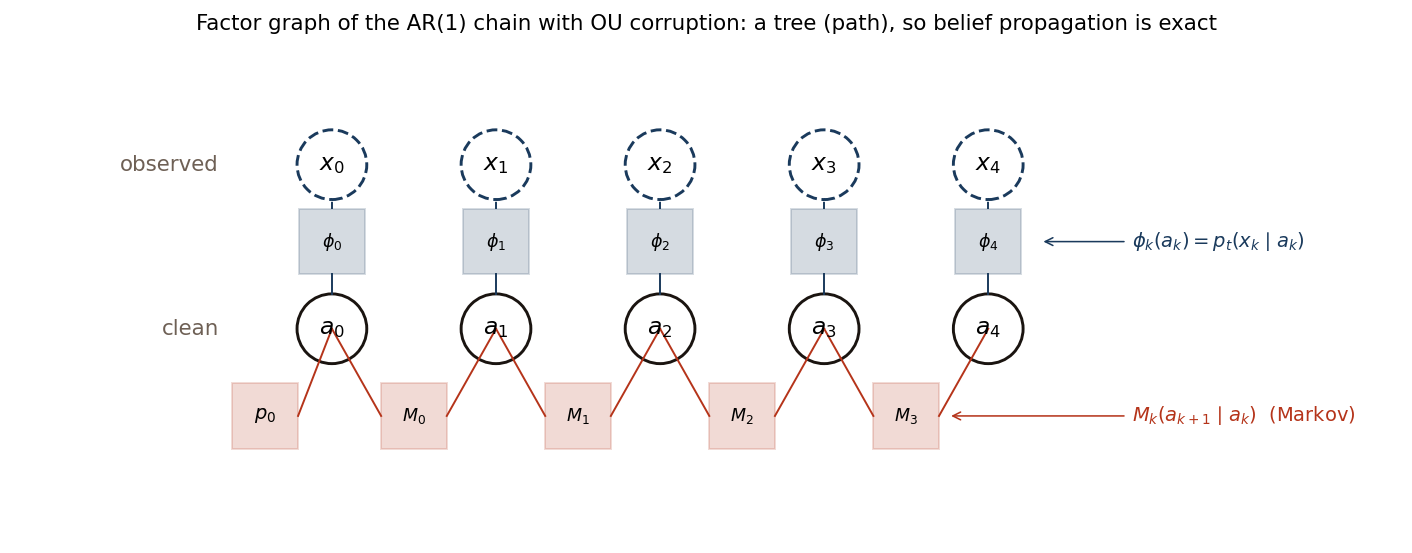
\includegraphics[width=\linewidth]{figures/fig02_factor_graph.png}
    \caption{Factor graph of the chain prior and OU likelihood.
    Solid edges connect clean variables \(a_k\) (white circles) to the
    prior factor \(p_0\) and the Markov transition factors
    \(M_k = M(a_{k+1} \mid a_k)\) (red squares). Dashed edges connect
    each clean variable to its local evidence factor
    \(\phi_k(a_k) = p_t(x_k \mid a_k)\) (navy squares) and through
    \(\phi_k\) to the observed \(x_k\) (dashed circle). The
    dependence among the \(a_k\) is a path; the local evidence factors
    have degree 1 from the \(a\)-side and add no edges among the
    \(a_k\); the graph is therefore a tree.}
    \label{fig:factor-graph}
\end{figure}

\begin{proposition}[Chain factor graph is a tree,
\Established]\label{prop:tree}
The factor graph of the posterior \eqref{eq:posterior-fact} is a tree.
\end{proposition}

\begin{derivation}[: counting edges and excluding cycles]
A tree on \(V\) nodes has exactly \(V - 1\) edges and no cycles. Our
factor graph has \(V = K\) variable nodes plus \(K\) local-evidence
factors plus \(K - 1\) transition factors plus 1 prior factor, hence
\(V = 3 K\). Edges: each transition factor contributes \(2\) edges
(\(K - 1\) factors \(\Rightarrow\) \(2 K - 2\) edges), each
local-evidence factor contributes \(1\) edge from \(a_k\)-side
(\(\Rightarrow K\) edges), the prior contributes 1 edge. Total:
\((2 K - 2) + K + 1 = 3 K - 1 = V - 1\). For acyclicity, observe that
the only structure that could form a cycle is among the variable
nodes mediated by transition factors; but successive transitions form
a path, not a cycle, because each \(M_k\) is connected only to its
two endpoints and the local-evidence and prior factors are leaves.
The graph is therefore connected (each \(a_k\) is reachable from
\(a_0\) by following transitions) with \(V - 1\) edges; it is a tree.
\end{derivation}

\begin{proposition}[Global Markov property,
\Established]\label{prop:global-markov}
Conditioning on any variable node \(a_k\) disconnects the graph into
two independent subtrees: the left sub-chain
\((a_0, \dots, a_{k - 1})\) together with their local evidence
\(x_0, \dots, x_{k - 1}\), and the right sub-chain
\((a_{k+1}, \dots, a_{K-1})\) together with their local evidence
\(x_{k+1}, \dots, x_{K-1}\). The two halves are conditionally
independent given \(a_k\).
\end{proposition}

\begin{derivation}[: cut-set argument]
Any path between an \(a_j\) with \(j < k\) and an \(a_\ell\) with
\(\ell > k\) in the factor graph must pass through \(a_k\) (the chain
is a path graph; there is no other route). Conditioning on \(a_k\)
removes \(a_k\) as an active node, severing every such path. The two
halves share no remaining factor; hence by the global Markov property
of factor graphs, they are conditionally independent given \(a_k\).
\end{derivation}

\begin{intuition}[: why the tree structure is what makes BP exact]
On a tree, marginalisation can be performed by sequential elimination
of leaves --- absorb a leaf into its unique neighbour, peel it off,
repeat. Each elimination step is a one-dimensional integral. The
sum--product algorithm \citep{Pearl1988, KschischangFreyLoeliger2001}
formalises this peeling into two passes (forward, backward), each
visiting every edge once. On a graph with cycles the same recursion
is not exact: information sent into the graph eventually returns,
doubly counted. The cycle-free structure of the chain factor graph is
exactly the absence of this double-counting -- which is why BP is
exact here.
\end{intuition}

% =============================================================================
\section{Belief propagation on the chain}\label{sec:bp}
% =============================================================================

We now derive belief propagation \citep{Pearl1988,
KschischangFreyLoeliger2001} on the chain factor graph in detail and,
in the Gaussian case, briefly note its identification with the Kalman
filter \citep{Kalman1960} and the Rauch--Tung--Striebel smoother
\citep{RauchTungStriebel1965}. The whole construction is rebuilt from
scratch -- earlier internal notes contained a double-counting trap
that we explicitly correct.

\subsection{Sum--product on the chain}

We adopt \emph{Convention~A}: the forward message at node \(k\)
carries the evidence \(x_0, \dots, x_{k - 1}\) only; the backward
message carries \(x_{k + 1}, \dots, x_{K - 1}\) only; the local
evidence \(p_t(x_k \mid a_k)\) is inserted at combination time, not
inside either recursion. This avoids double-counting any \(x_k\) and
is the only convention under which the simple combination rule
\eqref{eq:posterior-as-product} below holds.

\begin{proposition}[Convention~A messages,
\Established]\label{prop:convA}
Define
\begin{align}
    \mu_{\to 0}(a_0) &:= p_0(a_0), \label{eq:fwd-init}\\
    \mu_{\to k+1}(a_{k+1})
        &:= \int M(a_{k+1} \mid a_k)\, p_t(x_k \mid a_k)\,
                 \mu_{\to k}(a_k)\, \mathrm da_k, \label{eq:fwd-rec}\\
    \mu_{\leftarrow K-1}(a_{K-1}) &:= 1, \label{eq:bwd-init}\\
    \mu_{\leftarrow k - 1}(a_{k-1})
        &:= \int M(a_k \mid a_{k-1})\, p_t(x_k \mid a_k)\,
                 \mu_{\leftarrow k}(a_k)\, \mathrm da_k. \label{eq:bwd-rec}
\end{align}
Then for every \(k\),
\begin{equation}\label{eq:posterior-as-product}
    p(a_k \mid x) \;\propto\; \mu_{\to k}(a_k)\,
                              p_t(x_k \mid a_k)\,
                              \mu_{\leftarrow k}(a_k).
\end{equation}
\end{proposition}

\begin{derivation}[\ref*{prop:convA}: peeling the chain at \(a_k\)]
Start from the joint
\(P(a, x) = p_0(a_0) \prod_u M(a_{u+1} \mid a_u) \prod_j p_t(x_j \mid
a_j)\), and integrate out every \(a_j\) with \(j \neq k\). By the
global Markov property (Proposition~\ref{prop:global-markov}), this
integral splits into two independent halves at \(a_k\): the left half
involves \((a_0, \dots, a_{k - 1})\) and the evidence
\((x_0, \dots, x_{k - 1})\) with the prior \(p_0\); the right half
involves \((a_{k + 1}, \dots, a_{K - 1})\) and
\((x_{k + 1}, \dots, x_{K - 1})\). The local evidence factor at node
\(k\), \(p_t(x_k \mid a_k)\), depends only on \(a_k\) and on the
\emph{constant} \(x_k\); it factors out of both integrals.

\textbf{Left half.} Define recursively
\(\mu_{\to k}(a_k) := \int p_0(a_0) \prod_{u = 0}^{k - 1}
M(a_{u + 1} \mid a_u) \prod_{j = 0}^{k - 1} p_t(x_j \mid a_j)\,
\mathrm da_0 \cdots \mathrm da_{k - 1}\). Peeling off the leftmost
unintegrated variable, \(a_{k - 1}\),
\begin{align}
    \mu_{\to k}(a_k)
        &= \int M(a_k \mid a_{k - 1})\, p_t(x_{k - 1} \mid a_{k - 1})
                \nonumber \\
        &\qquad \times \biggl[
                \int p_0(a_0) \prod_{u = 0}^{k - 2}
                    M(a_{u + 1} \mid a_u) \prod_{j = 0}^{k - 2}
                    p_t(x_j \mid a_j)
                    \mathrm da_0 \cdots \mathrm da_{k - 2}
                \biggr] \mathrm da_{k - 1} \nonumber \\
        &= \int M(a_k \mid a_{k - 1})\, p_t(x_{k - 1} \mid a_{k - 1})\,
                \mu_{\to k - 1}(a_{k - 1})\, \mathrm da_{k - 1},
\end{align}
which is exactly the recursion \eqref{eq:fwd-rec}. The base case is
\eqref{eq:fwd-init} since when \(k = 0\) there is nothing to integrate
beyond the prior.

\textbf{Right half.} The analogous argument peeling from the right
gives \eqref{eq:bwd-rec}--\eqref{eq:bwd-init}. The base case
\(\mu_{\leftarrow K - 1} \equiv 1\) is uninformative: there is no
evidence to the right of the last frame.

\textbf{Combination.} The peeling left, multiplying by the unintegrated
local evidence \(p_t(x_k \mid a_k)\), and the peeling right give
exactly \eqref{eq:posterior-as-product}, with the proportionality
constant being \(P_t(x)\).
\end{derivation}

\begin{remark}[The double-counting trap]
A natural-looking but \emph{incorrect} alternative
(\emph{Convention~B}) absorbs the local evidence into the forward
message,
\(\mu_{\to k}^{\mathrm B}(a_k) := \mu_{\to k}^{\mathrm A}(a_k)\, p_t(x_k \mid a_k)\).
Under Convention~B the simple combination
\eqref{eq:posterior-as-product} double-counts \(x_k\) (once inside
\(\mu_{\to k}^{\mathrm B}\) and once at combination time) and must be
corrected by dividing by one local evidence factor. Convention~A is
the one that makes the textbook combination rule correct without
correction. The numerical audit
(section~\ref{sec:audit}) was decisive in pinning this down: under
Convention~A the BP score matches the matrix posterior to
\(10^{-14}\); under naive Convention~B the disagreement was
order-one.
\end{remark}

\subsection{Complexity}

\begin{computation}[: BP is \(O(K)\), brute force was \(O(K^2)\)]
Each pass (\eqref{eq:fwd-rec} or \eqref{eq:bwd-rec}) computes
\(K - 1\) messages, one per edge, via a single one-dimensional integral
each. The combination \eqref{eq:posterior-as-product} at every node is
a product of three one-variable functions followed by one
one-dimensional normalisation -- constant cost per node. The total
number of one-dimensional integrals is therefore
\begin{equation}\label{eq:bp-cost}
    \mathrm{cost}_{\mathrm{BP}}
    \;=\; \underbrace{(K - 1)}_{\text{forward}}
        + \underbrace{(K - 1)}_{\text{backward}}
        + \underbrace{K}_{\text{combine}}
    \;=\; O(K).
\end{equation}
This is the precise drop from the \(O(K^2)\) brute-force counting of
\eqref{eq:bf-cost}: BP saves a factor \(K\) by storing every
intermediate integral as a message and reusing it across all
marginals, instead of repeating it once per output marginal.
\end{computation}

\subsection{The Gaussian case: from BP to Kalman}\label{sec:bp-gaussian}

When \(P_0\) is Gaussian, every factor in the posterior
\eqref{eq:posterior-fact} is a Gaussian function of its variables, and
the BP recursions \eqref{eq:fwd-rec}--\eqref{eq:bwd-rec} preserve
Gaussianity: every message is itself Gaussian, parametrised by a
single \((m, v)\) pair per node. The forward recursion then reduces to
the predict--update cycle of the \emph{Kalman filter}
\citep{Kalman1960}, and the combination of forward and backward
passes reduces to the \emph{Rauch--Tung--Striebel smoother}
\citep{RauchTungStriebel1965}; we do not redo these classical
derivations here and refer to standard references
\citep{KschischangFreyLoeliger2001, Bishop2006} for the algebraic
details. The audit (\S\ref{sec:audit}) verifies our Convention-A
implementation \texttt{code/bp\_score.py} against an independent
matrix-form computation of \(\Sig_t^{-1}(x - \mu\,\mu_a)\) at machine
precision over 1600 configurations: in the Gaussian setting the BP
score coincides with the closed-form affine score of
Theorem~\ref{thm:affine-score}, exactly as the equivalence
``sum--product on a Gaussian chain \(\equiv\) Kalman filter and
smoother'' predicts.

\medskip\noindent
For the non-Gaussian case (\S\ref{sec:K1}, \S\ref{sec:K2}) Gaussian
closure breaks down and the messages must be tracked as
one-dimensional functions. The structural content of the recursions
\eqref{eq:fwd-rec}--\eqref{eq:bwd-rec} survives unchanged --- only
the parametrisation does not.

% =============================================================================
\section{Act~I --- Gaussian AR(1) benchmark}\label{sec:gaussian}
% =============================================================================

The Gaussian AR(1) chain is the only model in which the joint score
admits a complete closed-form treatment. We use it to disentangle two
structural properties that the literature often conflates:
\textbf{Gaussianity}, responsible for the \emph{linearity} of the
score, and \textbf{Markovianity}, responsible for the \emph{tridiagonal
sparsity} of the clean-time precision \(Q_0\).

\subsection{Clean covariance and tridiagonal precision}

\begin{proposition}[Stationary AR(1) covariance, \Established;
cf.\ \cite{BrockwellDavis1991}]\label{prop:stat-cov}
For the stationary Gaussian AR(1) chain on \(K\) frames,
\begin{equation}\label{eq:stat-covariance}
    \Sig_0[i, j] \;=\; \frac{\sigma_\eta^2}{1 - \alpha^2}\,
                        \alpha^{|i - j|}.
\end{equation}
\end{proposition}

\begin{derivation}[\ref*{prop:stat-cov}: unrolling the recursion]
By induction \(\E[a_u] = \alpha\, \E[a_{u - 1}] = 0\) for all \(u\),
since \(\E[\eta_u] = 0\) and \(a_0\) is centred. For \(u \geq u'\),
the AR(1) recursion unrolls as
\begin{equation}
    a_u \;=\; \alpha^{u - u'}\, a_{u'} \;+\; \sum_{j = 0}^{u - u' - 1}
              \alpha^j\, \eta_{u - j}.
\end{equation}
The innovation noise terms \(\eta_{u - j}\) are independent of
\(a_{u'}\) (they are indexed strictly after \(u'\)), so
\(\E[a_u\, a_{u'}] = \alpha^{u - u'}\, \E[a_{u'}^2]\). Stationarity
forces \(\E[a_{u'}^2] = \sigma_\eta^2 / (1 - \alpha^2)\) for every
\(u'\), hence the stated formula. By symmetry the same holds for
\(u < u'\) with \(|u - u'|\) replacing \(u - u'\).
\end{derivation}

\begin{proposition}[Tridiagonal clean precision, \Established]
\label{prop:Q0-tridiag}
The inverse \(Q_0 = \Sig_0^{-1}\) is exactly tridiagonal:
\begin{equation}\label{eq:Q0}
    Q_0[k, k] = \begin{cases}
        1 / \sigma_\eta^2, & k \in \{0, K - 1\}, \\
        (1 + \alpha^2) / \sigma_\eta^2, & 0 < k < K - 1,
    \end{cases}
    \qquad
    Q_0[k, k \pm 1] = -\alpha / \sigma_\eta^2,
\end{equation}
all other entries identically zero.
\end{proposition}

\begin{derivation}[\ref*{prop:Q0-tridiag}: from the joint log-density]
The Markov factorisation gives the joint log-density
\begin{equation}
    \log P_0(a)
        = -\frac{a_0^2}{2 \sigma_0^2}
        - \sum_{u = 0}^{K - 2} \frac{(a_{u + 1} - \alpha a_u)^2}{2 \sigma_\eta^2}
        + \text{const}.
\end{equation}
The matrix \(Q_0\) is the negative Hessian of \(\log P_0\) with respect
to \(a\). For the off-diagonals, only adjacent terms
\((a_{k+1} - \alpha a_k)^2\) couple \(a_k\) and \(a_{k+1}\); expanding
this term contributes a cross derivative \(-\alpha / \sigma_\eta^2\),
so \(Q_0[k, k + 1] = -\alpha / \sigma_\eta^2\) and entries at distance
\(\geq 2\) vanish.

For the diagonal at an interior \(k\) (\(0 < k < K - 1\)), \(a_k\)
appears in two transition terms, the left one
\((a_k - \alpha a_{k - 1})^2\) contributing \(1 / \sigma_\eta^2\) and
the right one \((a_{k + 1} - \alpha a_k)^2\) contributing
\(\alpha^2 / \sigma_\eta^2\), summing to
\((1 + \alpha^2) / \sigma_\eta^2\). At the left boundary \(k = 0\)
the prior contributes \(1 / \sigma_0^2\) and only the right transition
contributes \(\alpha^2 / \sigma_\eta^2\); using stationarity
\(\sigma_0^2 = \sigma_\eta^2 / (1 - \alpha^2)\) the sum simplifies to
\(1 / \sigma_\eta^2\). The right boundary \(k = K - 1\) is symmetric.
\end{derivation}

\begin{intuition}[: tridiagonality is Markovianity, not Gaussianity]
The argument used Gaussianity only to identify the precision with the
Hessian of \(-\log P_0\). The structure of the Hessian -- nonzero only
on first neighbours -- is purely a consequence of the chain
factorisation: each transition factor depends on at most two adjacent
variables. Any Markov chain with absolutely continuous transitions
has a log-density Hessian supported on the path graph; only its
\emph{values} depend on the specific transition law.
\end{intuition}

\begin{figure}[t]
    \centering
    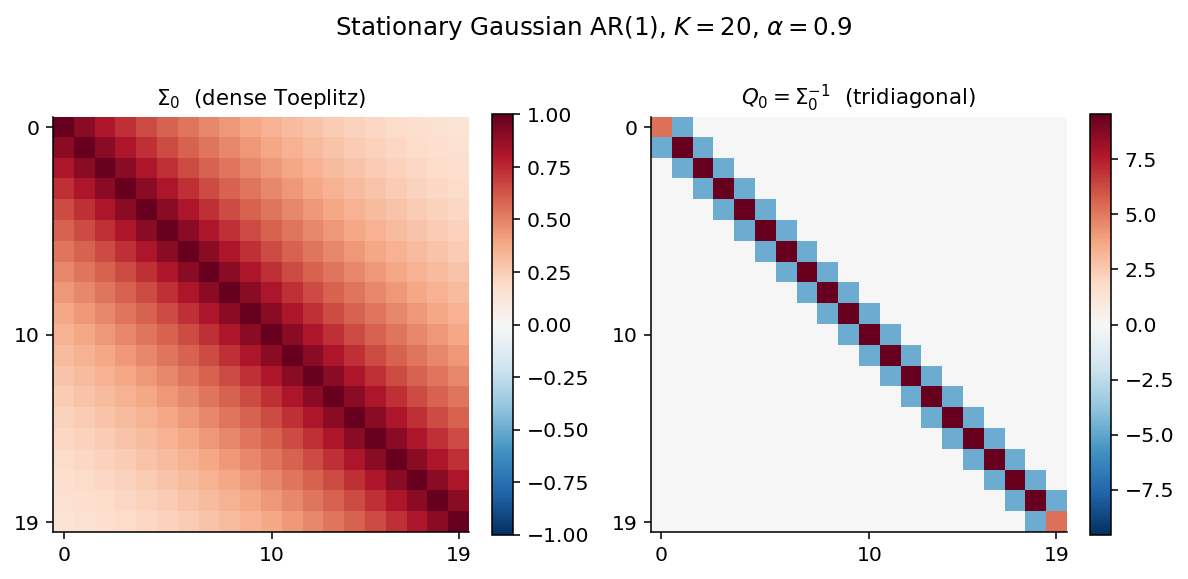
\includegraphics[width=0.95\linewidth]{figures/fig01_sigma_vs_precision.png}
    \caption{Stationary Gaussian AR(1), \(K = 20\), \(\alpha = 0.9\).
    Covariance \(\Sig_0\) (left) is dense Toeplitz with geometric
    off-diagonal decay; the inverse \(Q_0\) (right) is exactly
    tridiagonal. The only sparse object in the entire Gaussian story
    is \(Q_0\), and that sparsity is the algebraic shadow of the
    chain factorisation.}
    \label{fig:sigma-vs-precision}
\end{figure}

\subsection{Noised covariance and joint score}

\begin{proposition}[Noised covariance, \Established]
\(\Sig_t = \mu^2 \Sig_0 + \Detl\, I_K\).
\end{proposition}

\begin{derivation}[: the forward channel is a linear Gaussian map]
\(x = \mu a + \sqrt{\Detl}\, \xi\) with \(a \sim \mathcal N(0, \Sig_0)\)
and \(\xi \sim \mathcal N(0, I)\) independent. Independence of
\(a, \xi\) gives
\begin{equation}
    \Cov(x) = \mu^2\, \Cov(a) + \Detl\, \Cov(\xi) = \mu^2\, \Sig_0 + \Detl\, I.
\end{equation}
\end{derivation}

\begin{theorem}[Affine joint score, \Established]\label{thm:affine-score}
For Gaussian AR(1),
\begin{equation}
    S(x, t) \;=\; -\, Q_t\, (x - \mu\, \mu_a),
    \qquad Q_t = \Sig_t^{-1}, \qquad \mu_a[k] = \alpha^k \mu_0,
\end{equation}
which is exactly affine in \(x\) at every \(t\).
\end{theorem}

\begin{derivation}[\ref*{thm:affine-score}: from the Gaussian density]
\(P_t(x) = \mathcal N(x; \mu \mu_a, \Sig_t)\) gives
\(\log P_t(x) = -\tfrac{1}{2} (x - \mu \mu_a)^\top Q_t (x - \mu \mu_a) +
\text{const}\), whose gradient is \(-Q_t (x - \mu \mu_a)\).
\end{derivation}

Theorem~\ref{thm:affine-score} reduces every structural question about
the joint score to a question about the matrix \(Q_t\). The remainder
of this section describes \(Q_t\) in full closed form.

\subsection{Three equivalent representations of \(Q_t\)}

\begin{theorem}[Equivalent forms of \(Q_t\), \Established]\label{thm:three-forms}
For all \(t \geq 0\),
\begin{align}
    Q_t &= \tfrac{1}{\Detl}\, (I + \gamma_t\, \Sig_0)^{-1}, &
    \gamma_t &:= \tfrac{\mu^2}{\Detl}, \tag{SNR form} \label{eq:Qt-snr}\\
    Q_t &= U\, \mathrm{diag}\!\bigl( 1 / (\mu^2 \lambda_i + \Detl)\bigr) U^\top, &
    \Sig_0 &= U\, \mathrm{diag}(\lambda_i)\, U^\top, \tag{spectral form} \label{eq:Qt-spec}\\
    Q_t &= e^{2 t}\, Q_0\, (I + c_t\, Q_0)^{-1}
         = e^{2 t}\, \sum_{m \geq 0} (- c_t)^m Q_0^{m+1}, &
    c_t &:= e^{2 t} - 1. \tag{resolvent form} \label{eq:Qt-resolvent}
\end{align}
\end{theorem}

\begin{derivation}[\ref*{thm:three-forms}: three rewrites of the same identity]
\textbf{SNR form.} Factor \(\Detl\) out of \(\Sig_t = \mu^2 \Sig_0 +
\Detl I\) to write \(\Sig_t = \Detl (I + (\mu^2 / \Detl) \Sig_0) =
\Detl (I + \gamma_t \Sig_0)\), and invert.

\textbf{Spectral form.} Decompose \(\Sig_0 = U \mathrm{diag}(\lambda_i)
U^\top\). The identity matrix commutes with every basis change, so
\(\Sig_t = U \mathrm{diag}(\mu^2 \lambda_i + \Detl) U^\top\), and
\(Q_t = U \mathrm{diag}(1 / (\mu^2 \lambda_i + \Detl)) U^\top\). The
eigenvectors of \(\Sig_0\) are exactly the eigenvectors of \(\Sig_t\)
and \(Q_t\); only the eigenvalues evolve.

\textbf{Resolvent form.} Multiply \(\Sig_t = \mu^2 \Sig_0 + \Detl I\)
by \(Q_0\) to get \(Q_0 \Sig_t = \mu^2 I + \Detl Q_0\). Since
\(\mu^2 = e^{-2 t} = (1 + c_t)^{-1}\) and \(\Detl = 1 - \mu^2\), one
can verify by direct substitution that \(Q_t = e^{2 t} Q_0 (I + c_t
Q_0)^{-1}\). The Neumann series follows when \(\| c_t Q_0 \| < 1\),
which is the small-\(t\) regime where the SNR is high.
\end{derivation}

\begin{theorem}[Spectral preservation, \Established]\label{thm:spec-pres}
The eigenvectors of \(\Sig_t\) and \(Q_t\) coincide with those of
\(\Sig_0\) for every \(t \geq 0\); only the eigenvalues evolve, as
\(\lambda_i(t) = \mu^2\, \lambda_i + \Detl\). In the
\(\Sig_0\)-eigenbasis the multivariate denoising decouples into \(K\)
independent scalar denoisers.
\end{theorem}

\begin{intuition}[: locality is a basis-dependent statement]
Spectral preservation uses Gaussianity \emph{plus} isotropic noise --
no Markov structure is invoked. In the \(\Sig_0\)-eigenbasis,
\(Q_t\) is diagonal at every \(t\) -- maximally local. In the frame
basis, \(Q_t\) is tridiagonal only at \(t = 0\) -- as we will see, the
band fills with diffusion time. Both statements describe the same
matrix in different coordinates. The frame basis is the operationally
relevant one for video data.
\end{intuition}

\subsection{Lifecycle of the precision matrix}

The annotated heatmap in Figure~\ref{fig:precision-annotated} shows
the actual numerical values of \(Q_t\) at six diffusion times for
\(K = 6\), \(\alpha = 0.9\). Three regimes are visible:

\begin{itemize}[leftmargin=1.4em, topsep=2pt, itemsep=2pt]
\item \textbf{Tridiagonal (\(t \leq 10^{-5}\))}: the matrix is
indistinguishable from the clean \(Q_0\); off-band entries are at
floating-point noise (\(\sim 10^{-12}\)).
\item \textbf{Banded fill-in (\(10^{-3} \leq t \leq 10^{-1}\))}: the
distance-\(d\) entries grow as \(t^{d-1}\), with first neighbours
order one, second neighbours order \(t\), third neighbours order
\(t^2\), and so on.
\item \textbf{Identity floor (\(t \geq 1\))}: every entry decays
exponentially towards the identity at rate \(e^{-2 t}\); at \(t = 5\)
all off-diagonals are at \(\sim 10^{-5}\) and \(Q_t \approx I\) to
machine precision.
\end{itemize}

\begin{figure}[t]
    \centering
    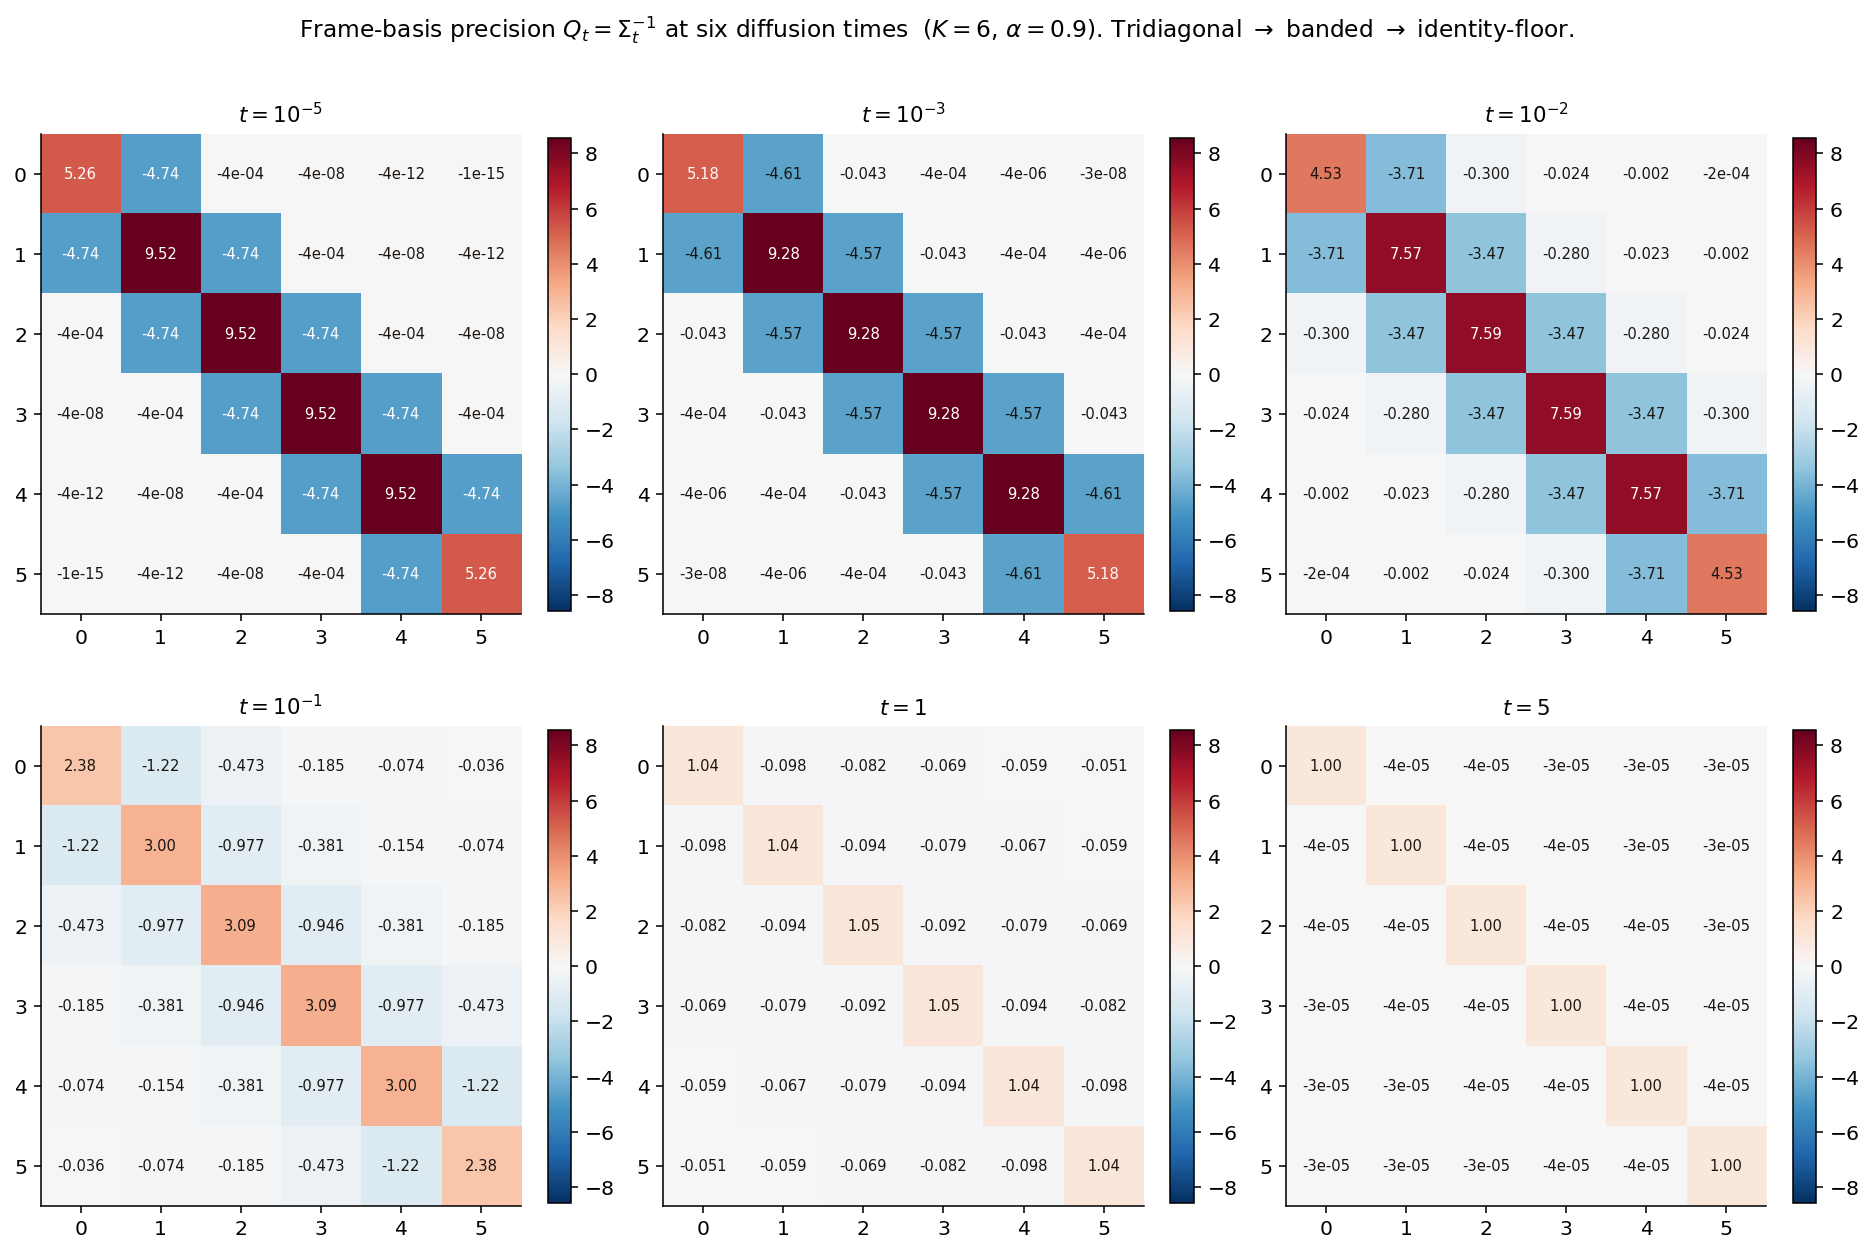
\includegraphics[width=\linewidth]{figures/fig03_precision_annotated.png}
    \caption{Frame-basis precision \(Q_t\) at six diffusion times,
    \(K = 6\), \(\alpha = 0.9\), with the actual numerical values
    written into every cell. Top row: \(t = 10^{-5}\) (effectively
    clean), \(t = 10^{-3}\), \(t = 10^{-2}\). Bottom row:
    \(t = 0.1\), \(t = 1\), \(t = 5\). The dense-to-sparse-to-identity
    lifecycle is visible directly in the entries: tridiagonal
    structure with \(\sim 9.5\) on the bulk diagonal and \(-4.7\) on
    the first off-diagonal at \(t = 10^{-5}\); weak distance-2 entries
    of order \(10^{-2}\) appearing already at \(t = 10^{-3}\); the
    matrix densifying through \(t = 10^{-1}\); collapsing toward the
    identity for \(t \geq 1\).}
    \label{fig:precision-annotated}
\end{figure}

\subsubsection{The band-fill theorem (corrected)}

The resolvent form \eqref{eq:Qt-resolvent} controls how the band fills
quantitatively. Powers of a tridiagonal matrix grow linearly in
bandwidth -- \(Q_0^m\) has bandwidth at most \(m\) -- so the
distance-\(d\) entry first appears at order \(t^{d-1}\):

\begin{theorem}[Band-fill leading order, \Established]\label{thm:band-fill}
For the Gaussian AR(1) precision under OU diffusion,
\begin{equation}\label{eq:band-fill}
    Q_t[i,\, i + d]
        \;=\; (-1)^{d - 1}\, (2 t)^{d - 1}\, (Q_0^d)_{i,\, i + d}
              \;+\; O(t^d).
\end{equation}
\end{theorem}

\begin{derivation}[\ref*{thm:band-fill}: small-\(t\) expansion of the resolvent]
Substitute \(c_t = 2 t + 2 t^2 + O(t^3)\) and \(e^{2 t} = 1 + O(t)\)
into the Neumann series \eqref{eq:Qt-resolvent}:
\begin{equation}
    Q_t \;=\; (1 + O(t))\,
              \bigl[\, Q_0 - c_t\, Q_0^2 + c_t^2\, Q_0^3 - \dots \,\bigr].
\end{equation}
The distance-\(d\) entry on the left receives contributions only from
matrix powers of bandwidth at least \(d\), i.e.\ \(Q_0^m\) with
\(m \geq d\). The smallest such power is \(m = d\), entering the
series with prefactor \((-c_t)^{d - 1}\). Substituting
\(c_t = 2 t (1 + t + O(t^2))\),
\((-c_t)^{d - 1} = (-1)^{d - 1} (2 t)^{d - 1} (1 + O(t))^{d - 1} =
(-1)^{d - 1} (2 t)^{d - 1} + O(t^d)\). Higher \(m\) contribute
\((-c_t)^{m - 1} = O(t^{m - 1})\) which is at least \(O(t^d)\). Hence
\eqref{eq:band-fill}.
\end{derivation}

\begin{remark}[Correction to a published formula]\label{rmk:correction}
An earlier internal note
(\texttt{precision\_lifecycle\_summary.pdf}, eq.~(12)) prints
\eqref{eq:band-fill} with an extraneous \(1 / (d - 1)!\) factor. That
factor does not follow from the resolvent expansion of equation~(10)
in the same note, and the audit
\texttt{numerical\_audit.py::check\_band\_fill} rejects it: the
no-factorial leading coefficient agrees with the empirical
\(Q_t[i, i + d] / t^{d - 1}\) to relative accuracy \(< 5\,\%\) for
\(d \in \{1, 2, 3, 4, 5\}\) at \(\alpha = 0.9\), \(K = 25\); the
factorial version fails the same test by orders of magnitude (errors
\(\sim 90\,\%\) at \(d = 3\), \(\sim 290\,\%\) at \(d = 4\),
\(\sim 800\,\%\) at \(d = 5\)). The proof sketch in the source PDF
itself reads ``the leading nonvanishing contribution at distance
\(d\) comes from the term \(m = d - 1\)'', which is consistent only
with the no-factorial formula.
\end{remark}

\begin{auditbox}[: band-fill verification]
\texttt{numerical\_audit.py::check\_band\_fill} compares the empirical
ratio \(Q_t[i, i+d] / t^{d-1}\) to the predicted leading coefficient
\((-1)^{d-1} 2^{d-1} (Q_0^d)_{i, i+d}\) for each \(d \in \{1, \dots,
5\}\), at the smallest \(t\) consistent with floating-point recovery
of the off-band entries. All five passes at relative tolerance \(5\,\%\).
The figure \texttt{fig04\_band\_fill.png}
(Figure~\ref{fig:band-fill}) plots \(|Q_t[i, i + d]|\) on log--log
axes against the corrected reference and confirms the match across
the small-\(t\) regime.
\end{auditbox}

\begin{figure}[t]
    \centering
    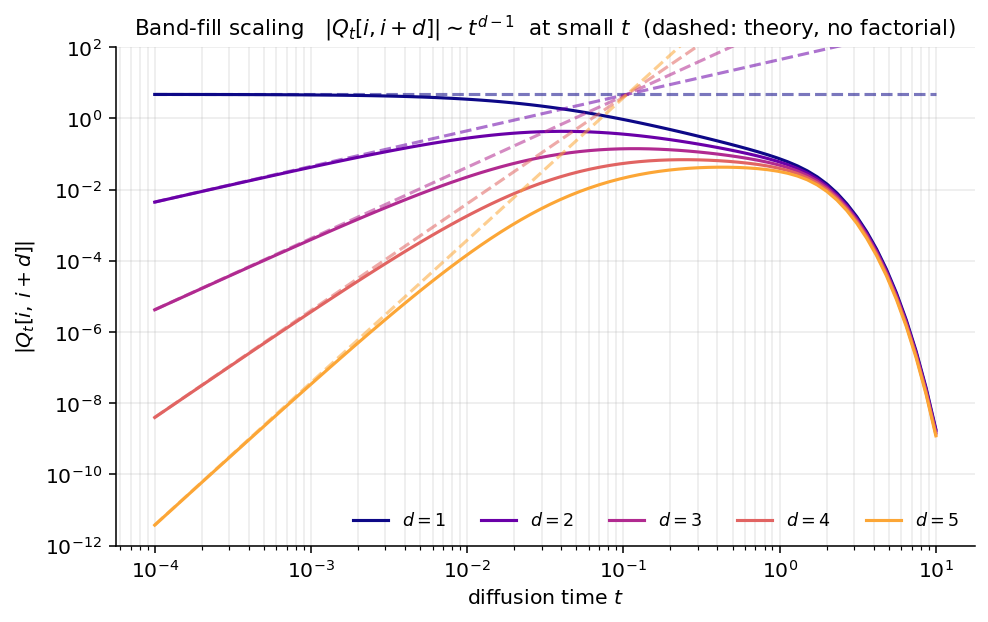
\includegraphics[width=0.7\linewidth]{figures/fig04_band_fill.png}
    \caption{Band-fill scaling. Solid: \(|Q_t[i, i + d]|\) for
    \(i = K/2\) and \(d = 1, \dots, 5\), computed by direct inversion
    of \(\Sig_t\). Dashed: corrected theoretical leading order
    \eqref{eq:band-fill} (no factorial). The match is exact at small
    \(t\); at \(t \gtrsim 1\) all curves bend over and decay together
    as \(Q_t\) returns to the identity.}
    \label{fig:band-fill}
\end{figure}

\subsubsection{Asymptotic exponential return to identity}

\begin{theorem}[Large-\(t\) asymptotic, \Established]\label{thm:large-t}
As \(t \to \infty\),
\begin{equation}
    Q_t \;=\; I - e^{-2 t}\, (\Sig_0 - I) + e^{-4 t}\, (\Sig_0 - I)^2
            + O(e^{-6 t}).
\end{equation}
\end{theorem}

\begin{derivation}[\ref*{thm:large-t}: Neumann at the identity]
Write \(\Sig_t = I + e^{-2 t}(\Sig_0 - I)\) (substituting
\(\mu^2 = e^{-2 t}\) and \(\Detl = 1 - e^{-2 t}\)). Apply
\((I + B)^{-1} = I - B + B^2 - \dots\) with \(B = e^{-2 t} (\Sig_0 -
I)\). The norm \(\|B\| = e^{-2 t} \|\Sig_0 - I\|\) is below 1 for
\(t\) large enough; the series converges and the first three terms
are as stated.
\end{derivation}

\subsection{The full-chain BP score recovers the matrix score}

Section~\ref{sec:bp} derived an \(O(K)\) algorithm for the joint
score by message passing. For Gaussian AR(1), the resulting score
must equal the closed-form expression of
Theorem~\ref{thm:affine-score}. The audit confirms this to machine
precision over 1600 configurations.

\begin{auditbox}[: BP vs matrix posterior, \(80\) configurations \(\times\) 20 random \(x\)]
\texttt{numerical\_audit.py::check\_bp\_vs\_matrix} sweeps
\(K \in \{2, 3, 5, 8, 16\}\), \(\alpha \in \{0.2, 0.5, 0.9, -0.4\}\),
\(t \in \{0.05, 0.3, 1.0, 3.0\}\), with 20 random \(x \sim \mathcal
N(0, I)\) per configuration. Maximum disagreements:
\begin{align*}
    \max\bigl|m_k^{\mathrm{BP}} - m_k^{\mathrm{matrix}}\bigr|
        &= 1.33 \times 10^{-15}, \\
    \max\bigl|v_k^{\mathrm{BP}} - \Sig_{\mathrm{post}}[k, k]\bigr|
        &= 3.89 \times 10^{-15}, \\
    \max\bigl|S_k^{\mathrm{BP}} - S_k^{\mathrm{matrix}}\bigr|
        &= 1.24 \times 10^{-14}.
\end{align*}
All three are at the level of double-precision rounding accumulated
through the recursion (\(K\) products of three Gaussians, each
introducing at worst one ULP).
\end{auditbox}

\begin{figure}[t]
    \centering
    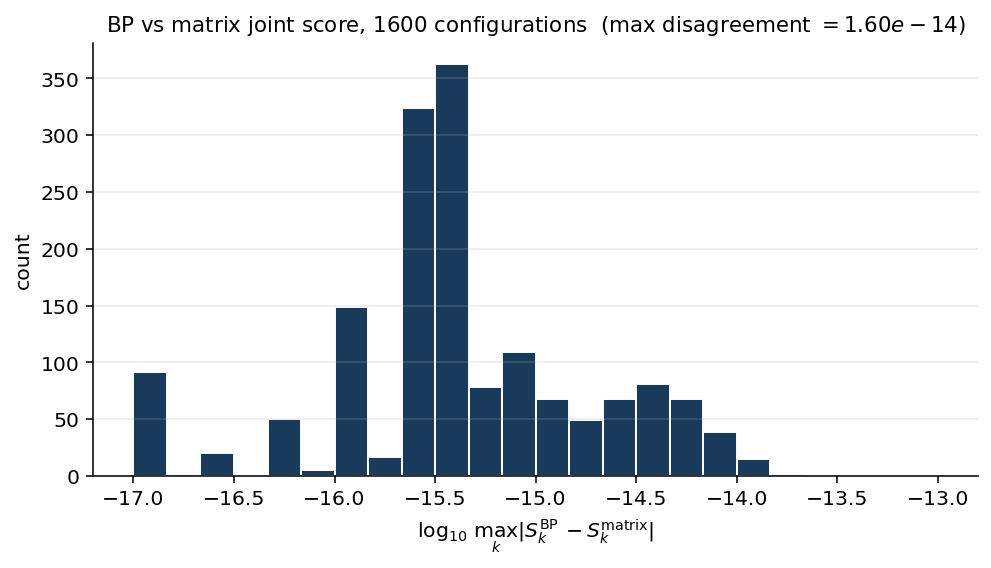
\includegraphics[width=0.7\linewidth]{figures/fig05_bp_audit.png}
    \caption{Histogram of \(\log_{10} \max_k |S_k^{\mathrm{BP}} -
    S_k^{\mathrm{matrix}}|\) over 1600 audit configurations. The bulk
    of residuals concentrates at \(\log_{10} \approx -15.5\)
    (machine-eps level for the score's magnitude); the leftmost
    floor bin is the clip at \(10^{-17}\) for configurations whose
    BP and matrix scores agree exactly to all displayed digits.}
    \label{fig:bp-audit}
\end{figure}

% =============================================================================
\section{Act~II --- Laplace warm-up at \(K = 1\)}\label{sec:K1}
% =============================================================================

For \(K = 1\) there is no chain and no Markov structure; the model
is the smallest case in which Tweedie's identity has to confront a
non-Gaussian prior. The clean variable is
\(a \sim \mathrm{Laplace}(0, b)\), \(p_0(a) = (1/2 b) e^{-|a|/b}\),
\(\Var(a) = 2 b^2\). The OU step yields
\(p_t(x) = \int p_0(a)\, \mathcal N(x; \mu a, \Detl)\, \mathrm da\).

\paragraph{Programme for the Laplace case (Garnier-Brun discussion).}
The current section and the next address three threads opened in
discussion with J\'er\^ome:
\begin{enumerate}[leftmargin=1.6em, topsep=2pt, itemsep=2pt]
\item express the joint score \(\score\) using the Markov structure of
the model;
\item rewrite the score in terms of \emph{relative} (innovation)
variables, making the dependence on the AR(1) shift explicit;
\item exploit a Fourier representation in which the noised marginal
satisfies a \emph{linear} ODE, recovering the \(K = 1\) building
block as a screened Poisson equation.
\end{enumerate}
Sections \ref{sec:K1-fourier} and \ref{sec:K1-curvature} address
threads 3 and (briefly) the resulting curvature observation for
\(K = 1\); section~\ref{sec:K2} addresses threads 1, 2, 3 for
\(K \geq 2\).

\begin{remark}[On the closed form]
The original note \texttt{session\_summary\_K1\_warmup.pdf} reduces
\(p_t(x)\) to a sum of two truncated-Gaussian terms (\S~3.3) using a
Mills-ratio asymptotic (Appendix~B). We \emph{omit} that derivation:
the closed form is convenient for board-work, but every quantitative
claim below is established by 1D quadrature in
\texttt{code/laplace\_score.py}, which is independent of the
truncated-Gaussian rewrite.
\end{remark}

\begin{computation}[: limits of the noised marginal]
\textbf{\(t \to 0\).} As \(\mu \to 1\) and \(\Detl \to 0\), the
Gaussian kernel \((2 \pi \Detl)^{-1/2} \exp[-(x - \mu a)^2 / 2 \Detl]\)
becomes a Dirac at \(a = x / \mu \to x\). The sifting property gives
\(p_0(x)\): the clean Laplace density is recovered.

\textbf{\(t \to \infty\).} As \(\mu \to 0\) and \(\Detl \to 1\), the
Gaussian kernel becomes \(a\)-independent and factors out, leaving
\(\int p_0(a)\, \mathrm da = 1\); hence \(p_\infty(x) = (2 \pi)^{-1/2}
\exp(-x^2 / 2)\), the standard normal attractor of the OU process.
\end{computation}

\begin{figure}[t]
    \centering
    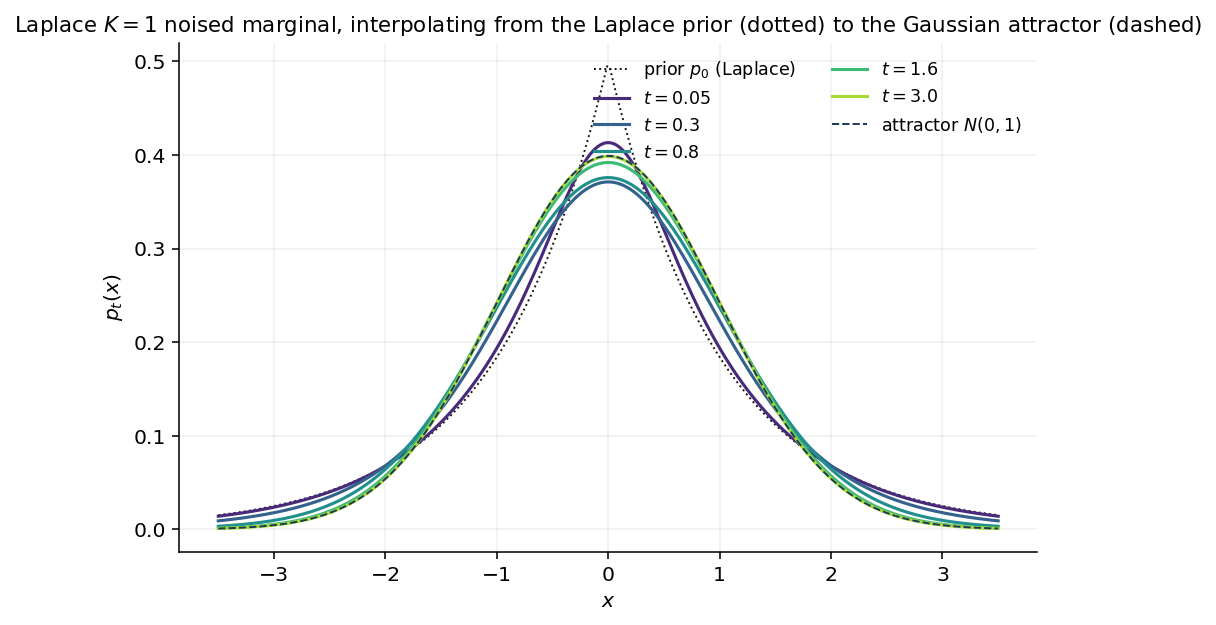
\includegraphics[width=0.78\linewidth]{figures/fig06_K1_density.png}
    \caption{Laplace \(K = 1\) noised marginal \(p_t^{(1)}(x)\)
    (\(b = 1\)) at increasing diffusion times. The dotted curve is
    the clean Laplace prior \(p_0(x) = \tfrac{1}{2} e^{-|x|}\); the
    dashed curve is the Gaussian attractor \(\mathcal N(0, 1)\). The
    family interpolates monotonically from the kinked Laplace shape
    at \(t \to 0\) to the smooth Gaussian at \(t \to \infty\).}
    \label{fig:K1-density}
\end{figure}

\subsection{The joint score acquires nonlinearity}

By Tweedie (Theorem~\ref{thm:tweedie}), \(S(x, t) = (\mu \E[a \mid x]
- x) / \Detl\); the score's \(x\)-dependence is exactly that of the
Bayesian denoiser.

\begin{intuition}[: where the nonlinearity lives]
For Gaussian \(p_0\), \(\E[a \mid x]\) is affine in \(x\) (Gaussian
conditioning), so the score is affine. For Laplace \(p_0\), the
conditional expectation is a smooth nonlinear interpolation between
the two limits below, and the score inherits the nonlinearity.
\end{intuition}

\begin{computation}[: limits of the joint score]
\textbf{\(t \to 0\).} Since \(p_t(x) \to p_0(x) = (1/2 b) e^{-|x|/b}\)
in the sense above, \(\partial_x \log p_t(x) \to -\mathrm{sign}(x) /
b\). The score per se diverges with \(\Detl^{-1}\); the rescaled
score \(\Detl S(x, t) \to -\mathrm{sign}(x) / b\) (up to the factor
\(b\) in our scaling). Figure~\ref{fig:K1-limits} (left) shows this
convergence for \(b = 1\).

\textbf{\(t \to \infty\).} As \(p_t(x) \to \mathcal N(0, 1)\), the
score \(\partial_x \log p_t(x) \to -x\): the Gaussian attractor of the
OU process. Figure~\ref{fig:K1-limits} (right) shows this convergence.
\end{computation}

\begin{figure}[t]
    \centering
    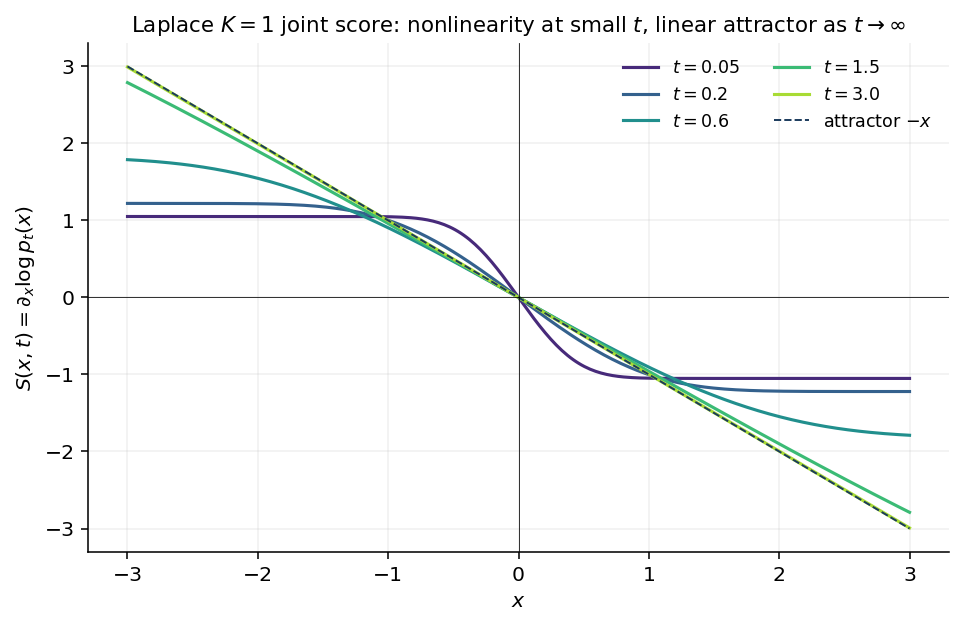
\includegraphics[width=0.78\linewidth]{figures/fig07_K1_score.png}
    \caption{Laplace \(K = 1\) joint score \(S(x, t) = \partial_x
    \log p_t(x)\) (\(b = 1\)) at the same diffusion times as
    Figure~\ref{fig:K1-density}; dashed line is the Gaussian attractor
    \(-x\). At small \(t\) the score saturates to a sign-like profile
    of magnitude \(\sim 1/b\); the nonlinearity sits in the kink near
    \(x = 0\) and progressively flattens out, recovering linearity as
    \(t \to \infty\).}
    \label{fig:K1-score}
\end{figure}

\begin{figure}[t]
    \centering
    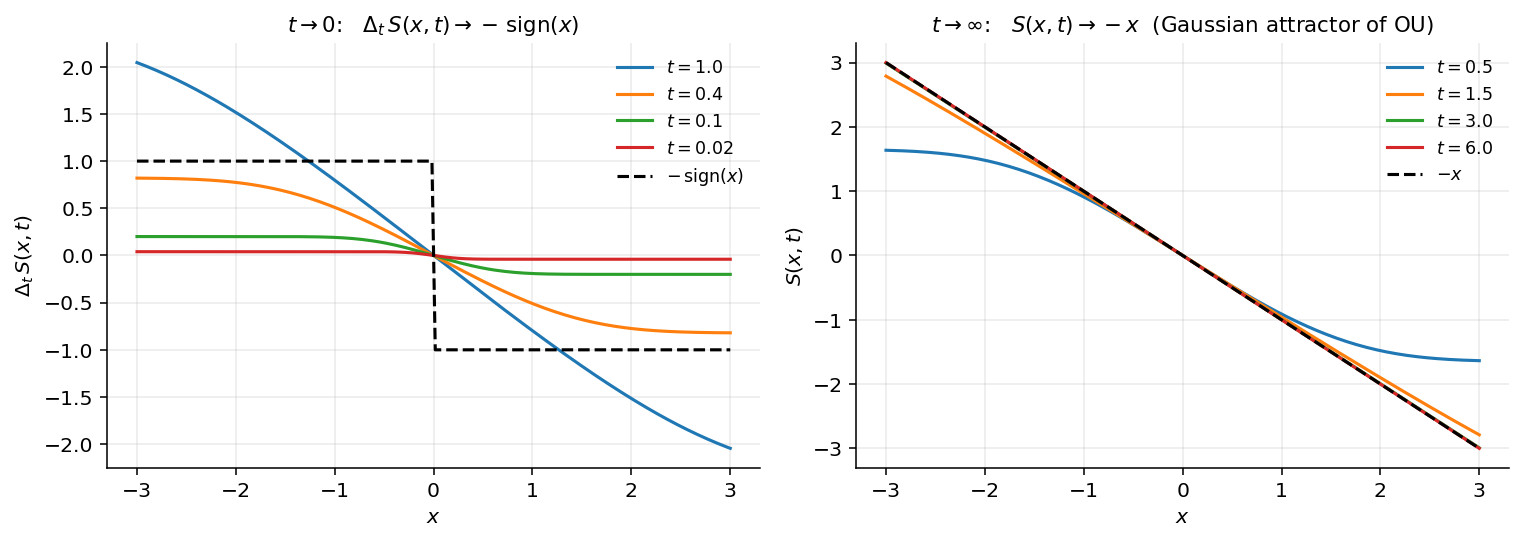
\includegraphics[width=\linewidth]{figures/fig08_K1_score_limits.png}
    \caption{Limits of the Laplace \(K = 1\) joint score
    (\(b = 1\)). Left: rescaled score \(\Detl S(x, t)\) for decreasing
    \(t\); the family converges pointwise to \(-\mathrm{sign}(x)\).
    Right: unscaled score for increasing \(t\); the family converges
    pointwise to \(-x\), the Gaussian attractor of the OU process.}
    \label{fig:K1-limits}
\end{figure}

\begin{auditbox}[: Tweedie versus finite difference]
\texttt{numerical\_audit.py::check\_laplace\_K1\_score\_fd} computes
the central finite difference of \(\log p_t\) at step \(h = 5 \times
10^{-4}\) for \((b, t, x) \in \{0.5, 1\} \times \{0.1, 0.4, 1, 2\}
\times \{-1, -0.3, 0.2, 0.7, 1.5\}\). The maximum disagreement against
Tweedie is \(1.19 \times 10^{-7}\), within the \(O(h^2)\) truncation
floor of the finite difference. The Gaussian-attractor limit at
\(t = 6\) is verified to \(7.4 \times 10^{-6}\).
\end{auditbox}

% -----------------------------------------------------------------------------
\subsection{Fourier representation: convolution becomes a
product}\label{sec:K1-fourier}
% -----------------------------------------------------------------------------

The forward channel \(y = \mu\, a + \sqrt{\Detl}\, \xi\) writes the
noised variable as the sum of two \emph{independent} random
variables: the rescaled clean signal \(\mu\, a\) and the channel noise
\(\sqrt{\Detl}\, \xi\). At the level of densities this independence
appears as a convolution, \(p_t^{(1)} = p_{\mu a} \star G_{\Detl}\),
where \(p_{\mu a}\) is the density of \(\mu a\) and
\(G_{\Detl}\) is the Gaussian of variance \(\Detl\). Convolutions are
hard to manipulate directly, but the Fourier transform turns them
into ordinary products: the characteristic function of a sum of
independent variables is the product of their characteristic
functions. That is the structural fact we now exploit.

\begin{theorem}[Characteristic-function factorisation, \Established]
\label{thm:K1-cf}
For \(a \sim \mathrm{Laplace}(0, b)\), \(\xi \sim \mathcal N(0, 1)\)
independent, and \(y = \mu\, a + \sqrt{\Detl}\, \xi\),
\begin{equation}\label{eq:K1-cf}
    \widehat p_t^{\,(1)}(k)
    \;=\; \underbrace{\frac{1}{1 + b^2 \mu^2 k^2}}_{\text{c.f. of }\mu a}
        \;\cdot\;
        \underbrace{e^{- \Detl\, k^2 / 2}}_{\text{c.f. of }\sqrt{\Detl}\,\xi}.
\end{equation}
\end{theorem}

\begin{derivation}[\ref*{thm:K1-cf}: convolution \(\leftrightarrow\) product]
\textbf{Step 1 --- the density of \(y\) is a convolution.} Because
\(\mu a\) and \(\sqrt{\Detl}\, \xi\) are independent, the density of
their sum is the convolution of their individual densities:
\begin{equation}
    p_t^{(1)}(y)
    \;=\; \int_{-\infty}^{+\infty}
            p_{\mu a}(y - z)\, G_{\Detl}(z)\, \mathrm dz
    \;=\; (p_{\mu a} \star G_{\Detl})(y).
\end{equation}

\textbf{Step 2 --- Fourier turns convolution into product.} The
convolution theorem states that the Fourier transform of a convolution
is the pointwise product of the individual transforms. Taking the
characteristic function (Fourier transform with conjugate sign
convention) of both sides,
\begin{equation}\label{eq:cf-product}
    \widehat p_t^{\,(1)}(k)
    \;=\;
    \widehat p_{\mu a}(k)\,\cdot\, \widehat G_{\Detl}(k).
\end{equation}
Independence of \(a\) and \(\xi\) is precisely what allows the joint
expectation \(\E[e^{i k y}] = \E[e^{i k (\mu a + \sqrt{\Detl}\, \xi)}]\)
to split into \(\E[e^{i k \mu a}]\, \E[e^{i k \sqrt{\Detl}\, \xi}]\),
which is \eqref{eq:cf-product} written out.

\textbf{Step 3 --- the two factors are standard characteristic
functions.} For \(a \sim \mathrm{Laplace}(0, b)\) with density
\(\tfrac{1}{2 b} e^{-|a|/b}\), a direct integral gives
\(\widehat p_a(k) = (1 + b^2 k^2)^{-1}\); rescaling by \(\mu\) sends
\(k \mapsto \mu k\), so
\(\widehat p_{\mu a}(k) = (1 + b^2 \mu^2 k^2)^{-1}\).
For \(\xi \sim \mathcal N(0, 1)\), \(\sqrt{\Detl}\, \xi \sim
\mathcal N(0, \Detl)\) and \(\widehat G_{\Detl}(k) = e^{-\Detl\,
k^2 / 2}\). Multiplying the two factors gives \eqref{eq:K1-cf}.
\end{derivation}

\begin{intuition}[: why working in Fourier is the right move]
In real space \(p_t^{(1)}\) is the convolution of a rough function
(Laplace, with a kink at \(0\)) with a smooth Gaussian; manipulating
the convolution directly forces one to confront the kink at every
step. In Fourier space the two factors of \eqref{eq:K1-cf} sit
\emph{side by side as a pointwise product}: any operation we apply on
the left ends up multiplying both factors. This is exactly what makes
the linear ODE below possible.
\end{intuition}

\begin{theorem}[Screened Poisson equation, \Established]\label{thm:screened-poisson}
The noised marginal \(p_t^{(1)}(y)\) satisfies the linear,
constant-coefficient ODE
\begin{equation}\label{eq:screened-poisson}
    \bigl(1 - b^2 \mu^2\, \partial_y^2\bigr)\, p_t^{(1)}(y)
    \;=\; G_{\Detl}(y),
    \qquad
    G_{\Detl}(y) \;:=\; \frac{1}{\sqrt{2 \pi \Detl}}\,
                         e^{-y^2 / (2 \Detl)}.
\end{equation}
\end{theorem}

\begin{derivation}[\ref*{thm:screened-poisson}: clearing the
denominator and undoing Fourier]
\textbf{Step 1 --- multiply both sides of \eqref{eq:K1-cf} by
\(1 + b^2 \mu^2 k^2\).} This removes the rational factor on the right:
\begin{equation}\label{eq:cleared-cf}
    \bigl(1 + b^2 \mu^2 k^2\bigr)\, \widehat p_t^{\,(1)}(k)
    \;=\; e^{- \Detl\, k^2 / 2}.
\end{equation}
The right-hand side is the characteristic function of the Gaussian
\(G_{\Detl}\), so its inverse Fourier transform is \(G_{\Detl}(y)\)
itself.

\textbf{Step 2 --- the differentiation rule \(k^2 \widehat f
\;\leftrightarrow\; -\partial_y^2 f\).} For any density \(f\) decaying
at infinity,
\(\widehat{(\partial_y f)}(k) = i k\, \widehat f(k)\); applying it
twice gives
\(\widehat{(\partial_y^2 f)}(k) = (i k)^2\, \widehat f(k) = - k^2\,
\widehat f(k)\). Inverting,
\begin{equation}\label{eq:k2-to-partial2}
    k^2\, \widehat f(k)
    \;\xleftrightarrow{\;\text{Fourier}\;}\;
    - \partial_y^2 f(y).
\end{equation}
\textbf{Second-order differentiation in real space corresponds to
multiplication by \(-k^2\) in Fourier space.} The minus sign is the
single fact that produces a sign change between the rational factor
\((1 + b^2 \mu^2 k^2)\) in Fourier and the differential operator
\((1 - b^2 \mu^2 \partial_y^2)\) in real space.

\textbf{Step 3 --- inverse-transform \eqref{eq:cleared-cf}
term by term.} The constant \(1\) on the left is the identity
operator. The \(b^2 \mu^2 k^2\) term, by \eqref{eq:k2-to-partial2},
corresponds to \(- b^2 \mu^2 \partial_y^2\). The Fourier inverse of
the right-hand side is \(G_{\Detl}(y)\). Combining,
\begin{equation}
    \bigl(1 - b^2 \mu^2\, \partial_y^2\bigr)\, p_t^{(1)}(y)
    \;=\; G_{\Detl}(y),
\end{equation}
which is \eqref{eq:screened-poisson}. \qed
\end{derivation}

\begin{intuition}[: a linear ODE with a Gaussian source]
\eqref{eq:screened-poisson} says that the noised Laplace marginal is
the solution of a second-order, linear, constant-coefficient ODE
driven by a Gaussian source. This is the structural advantage that
the Fourier representation extracts: a convolution of two distinct
densities in real space has been turned into the action of a single
local differential operator on \(p_t^{(1)}\). The operator
\((1 - b^2 \mu^2 \partial_y^2)\) is the inverse of the rational factor
\((1 + b^2 \mu^2 k^2)^{-1}\) in \eqref{eq:K1-cf}; the duality
\(k^2 \leftrightarrow -\partial_y^2\) is what allows it to be written
in this clean form. The further analysis of the ODE
\eqref{eq:screened-poisson} -- its Green's function, the
interpretation of \(b \mu\) as a screening length, the regimes
\(t \to 0\) and \(t \to \infty\) -- is a programme objective in its
own right and is not pursued in this note; \eqref{eq:screened-poisson}
is the structural statement we wanted.
\end{intuition}

\begin{auditbox}[: characteristic-function identity]
\texttt{numerical\_audit.py::check\_laplace\_K1\_fourier} verifies the
closed-form characteristic function \eqref{eq:K1-cf} numerically by
comparing it against a quadrature of the density against \(e^{i k y}\)
on \(b \in \{0.5, 1\}\), \(t \in \{0.2, 0.6, 1.4\}\),
\(k \in \{0.3, 1.0, 2.5\}\); maximum disagreement \(2.88 \times
10^{-6}\) at the floor of adaptive quadrature on an oscillatory
unbounded-domain integrand.
\end{auditbox}

% -----------------------------------------------------------------------------
\subsection{The curvature is \(x\)-dependent}\label{sec:K1-curvature}
% -----------------------------------------------------------------------------

Tweedie's identity (Theorem~\ref{thm:tweedie}) gives, by direct
differentiation of the score with respect to \(x\),
\begin{equation}\label{eq:H-tweedie}
    H_t(x) \;:=\; - \partial_x^2 \log p_t(x)
            \;=\; \frac{1}{\Detl}\, \biggl(1
                  - \frac{\mu^2}{\Detl}\, \Var\!\bigl[a \mid x\bigr]\biggr).
\end{equation}
For Gaussian \(p_0\), \(\Var[a \mid x]\) is a constant in \(x\)
(Gaussian conditioning has \(x\)-independent posterior variance), so
\(H_t\) is a constant -- the Hessian of an affine score. For Laplace
\(p_0\), the conditional variance is \(x\)-dependent, so \(H_t(x)\) is
a nontrivial \emph{field} on \(\R\). We do not develop the full
analysis of \(H_t(x)\) here -- it is a programme objective in its own
right, with quadrature-tractable expressions and bump-location
results that the dedicated \texttt{laplace\_ar1\_audit/} package
treats in detail. The point we want to record is simply that the
breakdown of \emph{Hessian constancy} is the second-order analogue of
the breakdown of \emph{score linearity}, and both follow from the
same source: a non-Gaussian prior turns
\(\E[a \mid x]\) into a nonlinear function of \(x\).

% =============================================================================
\section{Act~III --- Laplace AR(1) at \(K \geq 2\)}\label{sec:K2}
% =============================================================================

The Laplace AR(1) chain has joint density
\begin{equation}
    P_0(a) \;=\; \frac{1}{(2 b)^K}\,
        \exp\!\Bigl(-\tfrac{1}{b}\sum_{k=0}^{K-1} |a_k - \alpha a_{k-1}|\Bigr),
    \qquad a_{-1} := 0.
\end{equation}
The likelihood factorises across frames as in the Gaussian case, so
the posterior \(p(a \mid x)\) inherits the same chain factor graph.
Belief propagation is therefore still \emph{exact in principle}, but
the messages no longer remain Gaussian; computation requires either
1D quadrature or a tractable analytic representation. This section
addresses the three threads opened in section~\ref{sec:K1}: the
Markov-structured form of the score, its rewrite in relative
coordinates, and the Fourier programme that promotes the \(K = 1\)
screened Poisson identity \eqref{eq:screened-poisson} to a
recursive linear structure.

\subsection{The Markov-structured form of the joint score}\label{sec:K2-markov-score}

\begin{theorem}[Joint score from chain BP, \Established]
\label{thm:K2-markov-score}
For any chain prior \(P_0\) (in particular Laplace AR(1)) and the OU
likelihood, the joint score \(\score \in \R^K\) is given component-wise by
\begin{equation}\label{eq:K2-markov-score}
    S_k(x, t) \;=\; \frac{\mu\, \E[a_k \mid x] - x_k}{\Detl},
    \qquad
    \E[a_k \mid x] \;=\; \frac{\int a_k\, m_k(a_k)\, p_t(x_k \mid a_k)\,
                                 b_k(a_k)\, \mathrm da_k}
                              {\int m_k(a_k)\, p_t(x_k \mid a_k)\,
                                 b_k(a_k)\, \mathrm da_k},
\end{equation}
where \(m_k(a_k) := \mu_{\to k}(a_k)\) is the forward message and
\(b_k(a_k) := \mu_{\leftarrow k}(a_k)\) is the backward message of
section~\ref{sec:bp}, Convention~A.
\end{theorem}

\begin{derivation}[\ref*{thm:K2-markov-score}: Tweedie + sum--product]
Tweedie (Theorem~\ref{thm:tweedie}) gives
\(S_k(x, t) = (\mu \E[a_k \mid x] - x_k) / \Detl\). The conditional
expectation reduces to a single 1D integral via the marginal posterior
\(p(a_k \mid x) \propto m_k(a_k)\, p_t(x_k \mid a_k)\, b_k(a_k)\)
(Proposition~\ref{prop:convA}). The proportionality constant cancels
between the numerator and the denominator of the conditional
expectation, leaving the ratio of two one-dimensional integrals as
in \eqref{eq:K2-markov-score}.
\end{derivation}

\begin{intuition}[: this answers Jérôme's first thread]
\eqref{eq:K2-markov-score} is the explicit answer to ``express the
score using the Markov structure of the model.'' The cost is no
longer a \(K\)-dimensional integral of the joint posterior; it is two
one-dimensional message recursions plus one one-dimensional integral
per frame for the conditional expectation. For Gaussian
\(P_0\), the messages are Gaussian and the integrals collapse to
arithmetic on \((m, v)\) pairs (section~\ref{sec:bp}); for Laplace
\(P_0\), the messages are no longer Gaussian, but the
forward message still admits a clean closed form
(Proposition~\ref{prop:forward-K2}, below) that recycles the \(K = 1\)
screened-Poisson kernel.
\end{intuition}

\subsection{The boundary message has a clean closed form}\label{sec:K2-boundary}

The recursion \eqref{eq:bwd-rec} of Convention~A starts from the
uninformative \(\mu_{\leftarrow K - 1} \equiv 1\). Its first
iteration -- the step that combines the AR(1) transition with the
local evidence of a single frame against the trivial incoming message
-- has a clean closed form.

\begin{proposition}[One-step Laplace integral, \Established]\label{prop:forward-K2}
For the Laplace AR(1) transition
\(M(a' \mid a) = (1/2 b)\, e^{-|a' - \alpha a| / b}\) and the OU local
evidence \(p_t(x' \mid a') = \mathcal N(x';\, \mu a',\, \Detl)\),
\begin{equation}\label{eq:one-step-laplace}
    \int_{\R} M(a' \mid a)\, p_t(x' \mid a')\, \mathrm d a'
    \;=\;
    p_t^{(1)}\!\bigl(x' - \mu \alpha\, a\bigr),
\end{equation}
viewed as a function of \(a\), with \(p_t^{(1)}\) the universal
\(K = 1\) Laplace noised marginal of section~\ref{sec:K1}.
In particular, the first backward step of Convention~A (with
\(\mu_{\leftarrow k} \equiv 1\)) reads
\(\mu_{\leftarrow k-1}(a_{k-1}) = p_t^{(1)}(x_k - \mu \alpha\, a_{k-1})\).
\end{proposition}

\begin{derivation}[\ref*{prop:forward-K2}: change of variable to the
innovation]
Introduce the innovation variable \(r := a' - \alpha a\) (with \(a\)
held fixed). The transition density in this variable is
\(M(a' \mid a) = (1/2 b)\, e^{-|r| / b}\), i.e.\ the bare Laplace
prior of section~\ref{sec:K1} evaluated at \(r\). The Gaussian
likelihood at \(a' = \alpha a + r\) is
\(\mathcal N\!\bigl(x';\, \mu(\alpha a + r),\, \Detl\bigr)\),
which is just the OU kernel applied to the shifted argument
\(x' - \mu \alpha a\) at innovation \(r\). Marginalising \(r\) out,
\begin{equation}
    \int \tfrac{1}{2 b}\, e^{-|r|/b}\,
        \mathcal N\!\bigl(x';\, \mu(\alpha a + r),\, \Detl\bigr)\,
        \mathrm d r
    \;=\;
    \int p_0(r)\, \mathcal N\!\bigl(x' - \mu \alpha a;\, \mu r,\, \Detl\bigr)\,
        \mathrm d r
    \;=\;
    p_t^{(1)}\!\bigl(x' - \mu \alpha a\bigr),
\end{equation}
using the definition of the \(K = 1\) noised marginal. The shift
\(\mu \alpha a\) is precisely what frame \(a\) predicts for the next
frame's noised observation under the AR(1) dynamics, scaled by the
channel \(\mu\).
\end{derivation}

\subsection{General (non-boundary) messages have no clean form}\label{sec:K2-general}

\begin{remark}[Where the clean form breaks down, \Established
structurally]\label{rmk:causal-asym}
\eqref{eq:one-step-laplace} holds because the integrand involves
\emph{exactly one} Laplace kink (from \(M\)) multiplying \emph{exactly
one} Gaussian (from \(p_t(x' \mid a')\)). Any subsequent step of
either BP recursion --- in either direction --- breaks both
conditions: the message coming in carries the propagated structure of
several earlier frames, and is itself a sum of products of Laplace
kinks and Gaussian factors. The integrand at a general step is then a
product of \emph{two or more} absolute-value kinks with Gaussian
factors, which on each sign-quadrant reduces to a half-line Gaussian
but globally gives a sum of error functions whose argument depends on
the conditioning variable in a non-affine way. The closed form of the
boundary step does not survive iteration; this is the technical
content of the asymmetry between the Laplace and the Gaussian
benchmarks (in the Gaussian case every step is Gaussian-times-Gaussian
and the clean form propagates).
\end{remark}

\subsection{Innovation coordinates: prior factorises, likelihood
densifies}\label{sec:K2-innov}

The natural rewrite of the Laplace AR(1) prior is in terms of
\emph{innovation} variables that absorb the AR(1) shift. The result
makes the duality between prior and likelihood very explicit.

\begin{proposition}[Innovation factorisation, \Established]\label{prop:innov}
The triangular change of variables
\begin{equation}\label{eq:innov-def}
    r_0 \;=\; a_0,
    \qquad
    r_k \;=\; a_k - \alpha\, a_{k-1}
    \quad\text{for } k \geq 1,
\end{equation}
has unit Jacobian and decouples the prior into iid Laplace
coordinates:
\begin{equation}\label{eq:innov-prior}
    P_0(r) \;=\; \frac{1}{(2 b)^K}\, \prod_{k = 0}^{K - 1}
                 e^{-|r_k| / b}.
\end{equation}
Writing \(a = L\, r\) with \(L\) unit lower-triangular
(\(L_{ij} = \alpha^{i - j}\, \mathbf{1}_{i \geq j}\)), the OU
likelihood becomes
\begin{equation}\label{eq:innov-likelihood}
    p(x \mid r)
    \;\propto\;
    \exp\!\Bigl(- \tfrac{\mu^2}{2 \Detl}\,
        r^\top L^\top L\, r
        \;+\; \tfrac{\mu}{\Detl}\, x^\top L\, r\Bigr),
\end{equation}
and the matrix \(L^\top L\) is dense.
\end{proposition}

\begin{derivation}[\ref*{prop:innov}: change of variables in detail]
\textbf{Step 1 --- the inverse map is lower-triangular.} The defining
relations \eqref{eq:innov-def} read off the entries of \(r\) from
\(a\): \(r_0 = a_0\) and \(r_k = a_k - \alpha a_{k - 1}\). Reading them
the other way around, \(a_k = \alpha a_{k - 1} + r_k\), and unrolling
the recursion starting from \(a_0 = r_0\),
\begin{equation}
    a_k \;=\; \sum_{j = 0}^{k} \alpha^{k - j}\, r_j,
    \qquad k = 0, \dots, K - 1.
\end{equation}
This is \(a = L\, r\) with \(L_{ij} = \alpha^{i - j}\, \mathbf{1}_{i
\geq j}\); the diagonal is \(L_{ii} = 1\) so \(L\) is unit
lower-triangular and \(\det L = 1\).

\textbf{Step 2 --- the Jacobian of the change of variables is one.}
The Jacobian determinant of the linear map \(a = L r\) is
\(|\det L| = 1\), so the Lebesgue measure is invariant:
\(\mathrm d a = \mathrm d r\). Hence pushing forward any density
amounts to substituting \(a = L r\) without an extra factor.

\textbf{Step 3 --- the prior factor by factor.} The Laplace AR(1)
prior is
\(P_0(a) = (2 b)^{-K}\, \exp\!\bigl(-\tfrac{1}{b} \sum_{k}
|a_k - \alpha a_{k - 1}|\bigr)\) with \(a_{-1} := 0\). By
\eqref{eq:innov-def}, each kink \(|a_k - \alpha a_{k - 1}|\) is simply
\(|r_k|\); the \(k = 0\) term \(|a_0 - 0|\) is \(|r_0|\). Substituting
gives \eqref{eq:innov-prior}: a product of \(K\) iid Laplace densities.
The prior in \(r\)-coordinates is therefore as decoupled as it can
possibly be.

\textbf{Step 4 --- the likelihood in \(r\)-coordinates.} The OU
likelihood \(p(x \mid a) \propto \exp\!\bigl(-\tfrac{1}{2 \Detl}
\sum_k (x_k - \mu a_k)^2\bigr)\) is quadratic in \(a\), so
substituting \(a = L r\) gives
\begin{align}
    \sum_{k = 0}^{K - 1} (x_k - \mu a_k)^2
        &= \|x - \mu L r\|^2 \nonumber \\
        &= x^\top x \;-\; 2 \mu\, x^\top L r \;+\; \mu^2\, (L r)^\top (L r) \nonumber \\
        &= \mu^2\, r^\top L^\top L\, r \;-\; 2 \mu\, x^\top L\, r
                                       \;+\; \text{const}_r.
\end{align}
Dividing by \(2 \Detl\) and exponentiating gives
\eqref{eq:innov-likelihood}. The cost of decoupling the prior is the
cross term \(r^\top L^\top L\, r\): \(L^\top L\) is dense because the
unit-triangular \(L\) has all entries \(L_{ij} = \alpha^{i - j}\) in
its lower triangle, so
\((L^\top L)_{ij} = \sum_{m} L_{mi} L_{mj}\) sums geometric series
in \(\alpha\) and is non-zero for every pair \((i, j)\).
\end{derivation}

\begin{intuition}[: the AR(1) coupling cannot disappear]
The change to innovation coordinates is the cleanest possible
rewriting of the prior: it factorises completely into iid Laplace
variables. But the original AR(1) coupling did not vanish; it migrated.
In original coordinates the prior carried the chain coupling and the
likelihood was diagonal; in innovation coordinates the prior is
diagonal and the likelihood carries the coupling, through the dense
\(L^\top L\). There is no choice of basis in which both prior and
likelihood are diagonal simultaneously. The non-Gaussian counterpart
of the Gaussian observation in \S\ref{sec:gaussian} --- that
\(\Sig_t^{-1}\) is tridiagonal in the frame basis and diagonal in the
spectral basis, but never both --- is that the AR(1) shift has to live
somewhere.
\end{intuition}

\subsection{What the structure buys (and what is open)}

\Established\ Markovianity reduces the global \(K\)-dimensional
posterior expectation to two one-dimensional message recursions,
exactly as in the Gaussian case; computational locality survives.
The forward message is the universal \(K = 1\) noised density at a
shifted argument (Proposition~\ref{prop:forward-K2}), so the Act~II
analysis recycles as a building block.

\OpenTag\ A quadrature-tractable representation of the backward
message at \(K \geq 2\), or a controlled small-\(\alpha\) expansion,
would close the gap.

\OpenTag\ A precise, basis-independent statement of which
\emph{locality} of the joint score survives the non-Gaussian
extension. The candidates are sparsity of the position-dependent
Hessian \(H_t(x) = -\nabla_x^2 \log P_t(x)\) in some basis, low-rank
corrections to a tridiagonal core, or a perturbative expansion in
\(\alpha\) or in the strength of the non-Gaussianity. The earlier
project's quick-resolution low-rank conjecture
(\texttt{conjecture15\_test\_note.md}) is regime-dependent and pending
HPC verification; we do not commit to it here.

% =============================================================================
\section{Numerical audit summary}\label{sec:audit}
% =============================================================================

The driver \texttt{code/numerical\_audit.py} runs 53 closed-form-vs-reference
checks. The script exits non-zero if any check fails.
\textbf{As of compile date, 53/53 checks pass.}

\begin{auditbox}[: full check inventory]
\begin{tabular}{@{}p{0.62\linewidth} l l@{}}
\hline
Identity & max error & tolerance \\
\hline
Clean precision \(Q_0 = \Sig_0^{-1}\) (12 \((K, \alpha)\) configs)
    & \(1.78 \times 10^{-14}\) & \(10^{-12}\) \\
\(Q_0\) strictly tridiagonal, same configs
    & \(0\) & exact \\
\(\Sig_t\, Q_t = I\), 5 diffusion times
    & \(8.88 \times 10^{-16}\) & \(10^{-10}\) \\
\(Q_t\) direct vs spectral form, 5 times
    & \(2.22 \times 10^{-14}\) & \(10^{-10}\) \\
\(U\) diagonalises \(\Sig_0\), 5 times
    & \(1.19 \times 10^{-15}\) & \(10^{-10}\) \\
Band-fill leading coefficient, \(d \in \{1, \dots, 5\}\)
    (corrected formula \eqref{eq:band-fill})
    & \(2.7 \times 10^{-2}\) (rel.) & \(0.05\) (rel.) \\
\(\|Q_t - I\|_F\) vs large-\(t\) prediction, \(t \in \{3, 6, 10\}\)
    & \(2.08 \times 10^{-2}\) (rel.) & \(\propto e^{-2 t}\) \\
BP vs matrix posterior mean (80 configs)
    & \(1.33 \times 10^{-15}\) & \(10^{-10}\) \\
BP vs matrix posterior variance (80 configs)
    & \(3.89 \times 10^{-15}\) & \(10^{-10}\) \\
BP vs matrix joint score (80 configs)
    & \(1.24 \times 10^{-14}\) & \(10^{-10}\) \\
Tweedie matrix score self-consistency (Gaussian AR(1))
    & \(2.66 \times 10^{-15}\) & \(10^{-12}\) \\
Laplace \(K = 1\) score: Tweedie vs central FD
    & \(1.19 \times 10^{-7}\) & \(5 \times 10^{-7}\) \\
Laplace \(K = 1\) score \(\to -x\) at \(t = 6\)
    & \(7.37 \times 10^{-6}\) & \(10^{-3}\) \\
\hline
\end{tabular}
\end{auditbox}

% =============================================================================
\section{Closing argument: the factor graph as inductive bias}\label{sec:inductive-bias}
% =============================================================================

The previous sections established three connected facts. First,
Tweedie's identity (Theorem~\ref{thm:tweedie}) collapses the score to
the Bayesian denoiser \(\E[a \mid x]\), so the prior \(P_0\) enters
the score \emph{only} through this conditional expectation. Second,
the chain prior factorises \emph{and} the OU likelihood factorises,
so the posterior \(P(a \mid x)\) is a tree-structured graphical
model. Third, on a tree, sum--product is exact and runs in \(O(K)\),
identifying with the Kalman filter and the RTS smoother in the
Gaussian case. We close by drawing the architectural consequence.

\subsection{The intuition, made precise}

\begin{intuition}[: structure-aware versus universal-approximator priors]
The score-matching paradigm trains a neural network
\(s_\theta(x, t)\) to approximate \(\nabla_x \log P_t(x)\). The
network is a universal approximator: in absence of architectural
constraints, the prior over functions \(s_\theta\) it implements has
\emph{very high entropy} -- almost any reasonable smooth field can be
represented for some \(\theta\). The training data has to do all the
work of locating the right function in this enormous space.

For our problem, \(P_0\) is a stationary AR(1) chain. By
Theorem~\ref{thm:tweedie}, the score is determined by \(\E[a \mid x]\).
By Proposition~\ref{prop:posterior-fact}, \(\E[a_k \mid x]\) decomposes
through the chain factor graph. The forward and backward Kalman
recursions deliver \(\E[a_k \mid x]\) in \(O(K)\) operations, with no
training required (the recursion coefficients are functions of
\(\alpha, \sigma_\eta, t\), all known). Equivalently: the chain
structure of the prior \emph{is} a much more informative architectural
prior over score fields than ``unconstrained smooth'', and using it
collapses the model class to one that is exact for the assumed
generative model and \(O(K)\) to evaluate.
\end{intuition}

\subsection{The convolutional analogy}

A standard fully-connected MLP applied to images is a universal
approximator over functions of pixel vectors: it does not know that
the input is an image, that pixels have spatial neighbours, or that
visual patterns are typically translation-equivariant. Convolutional
networks bake exactly these facts into the architecture: local
filters, weight sharing, pooling. The result is a smaller hypothesis
class that contains the right answers for visual data, and that is
trainable from far fewer samples than the unstructured MLP would
require. The convolutional architecture \emph{is} an informative
prior; the training data is no longer asked to discover locality and
translation-equivariance, only to fit the residual.

Our setting is analogous, with locality of \emph{visual} pattern
replaced by locality of \emph{temporal} dependence. The information we
have about the data-generating process -- that it is a stationary
Markov chain under known iid Gaussian corruption -- is exactly the
information that converts a generic score-field hypothesis class into
the sum--product algorithm on the chain factor graph. Implementing
the score model as that algorithm:

\begin{itemize}[leftmargin=1.4em, itemsep=2pt]
\item \textbf{Reduces the parameter count} from a generic neural
score field (millions of weights) to the AR(1) transition parameters
\((\alpha, \sigma_\eta, p_0)\) plus, in the non-Gaussian case, a
finite-dimensional parametrisation of the messages.
\item \textbf{Reduces the inference cost} from a forward pass through
a deep network to two \(O(K)\) sequential passes whose total scalar
arithmetic is comparable to a few attention layers but with provable
exactness in the Gaussian case.
\item \textbf{Provides a controlled non-Gaussian extension}. Section
\ref{sec:K2} shows the chain factor graph survives non-Gaussian
priors; the only obstruction is the analytic representation of
non-Gaussian messages, which is the right hard problem to attack
next.
\end{itemize}

\begin{intuition}[: the programme objective in one line]
Replace the universal-approximator score model with a
factor-graph score model whose architecture mirrors the Markov
structure of the prior. Train the latter, when training is needed,
only on the residual that is not already captured by the chain
factorisation.
\end{intuition}

\subsection{Open programme directions}

\begin{enumerate}[leftmargin=1.4em]
\item Quadrature-tractable backward message at \(K \geq 2\) for the
Laplace prior, possibly via a Fourier or screened-Poisson
representation borrowed from the \(K = 1\) analysis.
\item Explicit connection between the joint propagator
\(P_t : S_{k - 1}(x, t) \mapsto S_k(x, t)\) and the Kalman gain in
the Gaussian case; quantification of when an approximate \(P_t\)
extracted from the exact Gaussian solution is a useful inductive bias
for non-Gaussian chains. The dynamical-regime picture of
\cite{Biroli2024} suggests this question is sharpest near the
speciation transition.
\item Empirical comparison: on a synthetic AR(1)-with-Laplace-noise
benchmark, train a generic temporal U-Net score model and compare
sample quality, compute, and parameter count against a
factor-graph-structured score with the same training budget.
\end{enumerate}

% =============================================================================
\section*{Reproducibility}
\addcontentsline{toc}{section}{Reproducibility}
% =============================================================================

The \texttt{code/} directory contains five modules:

\begin{description}[leftmargin=1.4em, style=nextline]
\item[\texttt{ar1\_utils.py}] Stationary AR(1) covariance and tridiagonal
precision; OU forward channel; \(\Sig_t\) and \(Q_t\) (direct and
spectral); affine joint score; matrix Gaussian posterior used by the
audit.
\item[\texttt{bp\_score.py}] Belief propagation under Convention~A;
forward (Kalman filter) and backward (RTS smoother) recursions;
posterior mean and joint score via Tweedie. Handles the
uninformative initial backward message exactly through
\(v = +\infty\).
\item[\texttt{laplace\_score.py}] \(K = 1\) Laplace warm-up: noised
marginal, posterior mean, and joint score by 1D quadrature; Gaussian
\(K = 1\) reference for side-by-side comparisons.
\item[\texttt{numerical\_audit.py}] 53 independent checks against
analytic, matrix, finite-difference, and quadrature references;
exits non-zero if any check fails.
\item[\texttt{generate\_figures.py}] Reproduces all 8 PNGs of this
note deterministically.
\end{description}

To reproduce:
\begin{verbatim}
cd Score_Diffusion/Research/unified_document/code
python3 numerical_audit.py    # MUST report 53/53 PASSED
python3 generate_figures.py   # writes ../figures/fig0{1..8}_*.png
cd ..
tectonic main.tex             # preferred: single-binary engine
# or:  pdflatex main.tex && pdflatex main.tex
\end{verbatim}

The Python stack is \texttt{numpy + scipy + matplotlib} only; no
neural network or stochastic training code appears anywhere in the
pipeline.

% =============================================================================
\addcontentsline{toc}{section}{References}
\bibliographystyle{plainnat}
\bibliography{references}
% =============================================================================

\end{document}
